\documentclass[a4paper,11pt,spanish, twoside, leqno]{tfg-uam}

\usepackage[utf8]{inputenc}
\usepackage{amsfonts, amssymb, amsmath, amsthm}
\usepackage{graphicx}
\usepackage{color}
\usepackage{xcolor}
\usepackage{tikz}
\usepackage{listofitems} % for \readlist to create arrays
\usepackage{hyperref}
\usepackage{algorithmic}
\usepackage{algorithm}
\usepackage{mdframed}
\usepackage{marginnote}
\usepackage[backend=bibtex, style=numeric]{biblatex} 
\usepackage{listings}
\usepackage{xcolor}

\DeclareMathOperator*{\argmax}{arg\,max}
\DeclareMathOperator*{\argmin}{arg\,min}

% Define custom colors for syntax highlighting
\definecolor{codegreen}{rgb}{0,0.6,0}
\definecolor{codegray}{rgb}{0.5,0.5,0.5}
\definecolor{codepurple}{rgb}{0.58,0,0.82}
\definecolor{backcolour}{rgb}{0.95,0.95,0.92}

% Customize the look of the code
\lstdefinestyle{mystyle}{
    backgroundcolor=\color{backcolour},   
    commentstyle=\color{codegreen},
    keywordstyle=\color{magenta},
    numberstyle=\tiny\color{codegray},
    stringstyle=\color{codepurple},
    basicstyle=\ttfamily\footnotesize,
    breakatwhitespace=false,         
    breaklines=true,                 
    captionpos=b,                    
    keepspaces=true,                 
    numbers=left,                    
    numbersep=5pt,                  
    showspaces=false,                
    showstringspaces=false,
    showtabs=false,                  
    tabsize=2
}

% Apply the style to listings
\lstset{style=mystyle}

\addbibresource{references.bib} % Link to your .bib file


\mdfsetup{%
linecolor=white,
backgroundcolor=gray!10,
}
\tikzstyle{mynode}=[thick,draw=black,fill=blue!20,circle,minimum size=18]

\newtheorem{teor}{Teorema}[chapter]
\newtheorem{lema}[teor]{Lema}
\newtheorem*{teorsin}{Teorema}


\renewcommand*{\raggedrightmarginnote}{\raggedright}

\theoremstyle{definition}
\newtheorem{defin}[teor]{Definici\'on}
\newtheorem{exmp}[teor]{Ejemplo}
\newtheorem{dem}[teor]{Demostración}

\title{Redes Neuronales: Aproximación de EDPs}
\author{Luis Hebrero Garicano}
\tutor{Julia Novo}
\curso{2024-2025}




%%%%%METADATOS: rellenar la info solicitada entre llaves
\usepackage{hyperref}
\hypersetup{
	pdfinfo={
            Title={Redes Neuronales: Aproximacion de EDPs}, %Titulo del trabajo; ejemplo: Matemáticas y desarrollo
            Author={Luis Hebrero Garicano}, %Autor del trabajo; ejemplo: Juan Sanchez
            Director1={julia.novo}, %Tutor1: en formato nombre.apellido, tal como aparece en la primera parte, antes de la arroba,  de su direcci�n de correo electr�nico de la UAM; ejemplo: fernando.soria
            Director2={ }, %Tutor2: en formato nombre.apellido, tal como aparece en la primera parte, antes de la arroba,  de su direcci�n de correo electr�nico de la UAM
            Ndirectores={1}, %Numero total de directores: 1 � 2
            Tipo={TFG}, %no tocar
            Curso={2024-25}, %no tocar
            Palabrasclave={ },% Palabras clave del trabajo, separadas por comas y sin acentos ni espacios; ejemplo: morfismos, formas modulares, ecuaciones elípticas
				}
}
%%%%%%%%%%%%%%%%%%%%%%%%%%%%%%%

\begin{document}



\begin{abstract}[spanish]
Las redes neuronales son un modelo matemático inspirado en el funcionamiento cerebral que, en esencia, se utiliza para encontrar funciones: funciones que clasifican datos, que predicen valores o incluso que anticipan la siguiente palabra en una frase. En este trabajo, se estudiará cómo se puede aplicar esta capacidad de aproximación de funciones para resolver ecuaciones en derivadas parciales. Exploraremos distintas estrategias para construir estas redes y analizaremos su aplicación en problemas concretos, centrándonos en las ventajas que aportan con respecto a los métodos numéricos tradicionales, así como en los casos en los que una aproximación mediante redes neuronales no resulta efectiva.
\end{abstract}
\begin{abstract}[english]
Neural networks are a mathematical model inspired by the brain's functioning, primarily used to find functions: functions that classify data, predict values, or even anticipate the next word in a sentence. This work will explore how this function approximation capability can be applied to solve partial differential equations. We will investigate different strategies for constructing these networks and analyze their application to specific problems, focusing on the advantages they offer over traditional numerical methods, as well as the cases where a neural network-based approach proves ineffective.
\end{abstract}
\mainmatter


\chapter{Introducción y preliminares}\label{chap1}
\setcounter{page}{1}
Para poder entender las aproximaciones a las EDPs mediante redes neuronales, es necesario tener un conocimiento previo de las redes neuronales y de las ecuaciones en derivadas parciales. En este capítulo, se introducirán los conceptos básicos de ambos temas, así como las herramientas matemáticas necesarias para comprender el resto del trabajo.

\section{Introducción a las redes neuronales}\label{sec:RedesNeuronales}
Una red neuronal, de forma abstracta, es simplemente una función que toma una entrada y produce una salida. Es decir, una red neuronal, es una función $F$ que toma un vector de entrada $x$ y produce un vector de salida $y$, siendo $F: \mathbb{R}^n \rightarrow \mathbb{R}^m$. La red neuronal se compone de una serie de capas, cada una de las cuales está formada por un conjunto de neuronas. Cada neurona de una capa recibe una serie de entradas, las procesa y produce una salida. La salida de cada neurona se calcula mediante una función de activación, que puede ser de distintos tipos, como la función sigmoide, la función tangente hiperbólica o la función ReLU. Para entender este concepto nos vamos a centrar en el caso concreto de la red neuronal de la Figura \ref{fig:RedNeuronal}.


\begin{figure}
    \centering
    \begin{tikzpicture}[x=2.2cm,y=1.4cm]
        \readlist\Nnod{2,2,3,3} % number of nodes per layer
        \readlist\colors{mylightred, mylightblue, mylightblue, mylightgreen} % color of each layer
        % \Nnodlen = length of \Nnod (i.e. total number of layers)
        % \Nnod[1] = element (number of nodes) at index 1
        \foreachitem \N \in \Nnod{ % loop over layers
          % \N     = current element in this iteration (i.e. number of nodes for this layer)
          % \Ncnt  = index of current layer in this iteration
          \foreach \i [evaluate={\x=\Ncnt; \y=\N/2-\i+0.5; \prev=int(\Ncnt-1);}] in {1,...,\N}{ % loop over nodes
            \node[mynode] (N\Ncnt-\i) at (\x,\y) {};
            \ifnum\Ncnt>1 % connect to previous layer
              \foreach \j in {1,...,\Nnod[\prev]}{ % loop over nodes in previous layer
                \draw[thick] (N\prev-\j) -- (N\Ncnt-\i); % connect arrows directly
              }
            \fi % else: nothing to connect first layer
          }
        }
    \end{tikzpicture}
    \caption{Esquema de una red neuronal con 4 capas.}
    \label{fig:RedNeuronal}
\end{figure}

Como se ve en la Figura \ref{fig:RedNeuronal}, la entrada en nuestra función está representada por los dos círculos de la izquierda, que representan los valores de entrada $x_1$ y $x_2$, siendo así la entrada $x\in\mathbb{R}^2$. Estos valores se multiplican por unos pesos ($W^{[2]}$)y se suman a un sesgo $b^{[2]}$. La salida de esta neurona se calcula mediante una función de activación. Así, los valores que ``llegan'' a la segunda capa de nuestra red neuronal serán de la forma
\begin{equation*}
    \sigma(W^{[2]}x+b^{[2]})\in\mathbb{R}^2,
\end{equation*}

Siendo $W^{[2]}\in\mathbb{R}^{2\times2}$ y el vector $b^{[2]}\in\mathbb{R}^2$. A partir de aquí, se repite el proceso para cada capa de la red neuronal, hasta llegar a la capa de salida, que nos dará el valor de salida de nuestra red neuronal. De forma visual, se pueden interpretar las líneas de la Figura \ref{fig:RedNeuronal} como los pesos por los que se va multiplicando.

En la tercera capa de la red neuronal, vemos que los valores que llegan de la capa 2, estos $\sigma(W^{[2]}x+b^{[2]})$, pertenecen a $\mathbb{R}^2$. De este modo, como tenemos 3 neuronas en la tercera capa, para obtener un valor perteneciente a $\mathbb{R}^3$, necesitamos una matriz $W^{[3]}\in\mathbb{R}^{3\times2}$ y un vector $b^{[3]}\in\mathbb{R}^3$. Así, el valor de nuestra red neuronal en la tercera capa será
\begin{equation*}
    \sigma(W^{[3]}\sigma(W^{[2]}x+b^{[2]})+b^{[3]})\in\mathbb{R}^3.
\end{equation*}

Finalmente, la capa de salida recibirá de la tercera capa un vector perteneciente a $\mathbb{R}^3$, por lo que necesitaremos una matriz $W^{[4]}\in\mathbb{R}^{3\times3}$ y un vector $b^{[4]}\in\mathbb{R}^3$. Así, el valor de salida de nuestra red neuronal, esa $F$ de la que habíamos hablado al principio, será
\begin{equation}
    F(x)=\sigma(W^{[4]}\sigma(W^{[3]}\sigma(W^{[2]}x+b^{[2]})+b^{[3]})+b^{[4]})\in\mathbb{R}^3.
\end{equation}\label{eq:RedNeuronal}

En general, una red neuronal se puede representar como una composición de funciones, donde cada función es una capa de la red neuronal. 

Nuestra intención con este tipo de funciones es ir variando los valores de las matrices $W$, también conocidos como pesos, y los vectores $b$ también conocidos como sesgos, para que la salida de nuestra red neuronal se acerque lo máximo posible a la salida deseada. 

Para entender esto, vamos a utilizar la red neuronal de la Figura \ref{fig:RedNeuronal} para resolver un problema concreto muy sencillo de clasificación. Supongamos que tenemos una serie de puntos en el plano, de tres tipos distintos, como los de la Figura \ref{fig:Clasificacion}, y queremos clasificarlos en tres grupos, los puntos de tipo azul, rojo y verde.


\begin{figure}
    \centering
    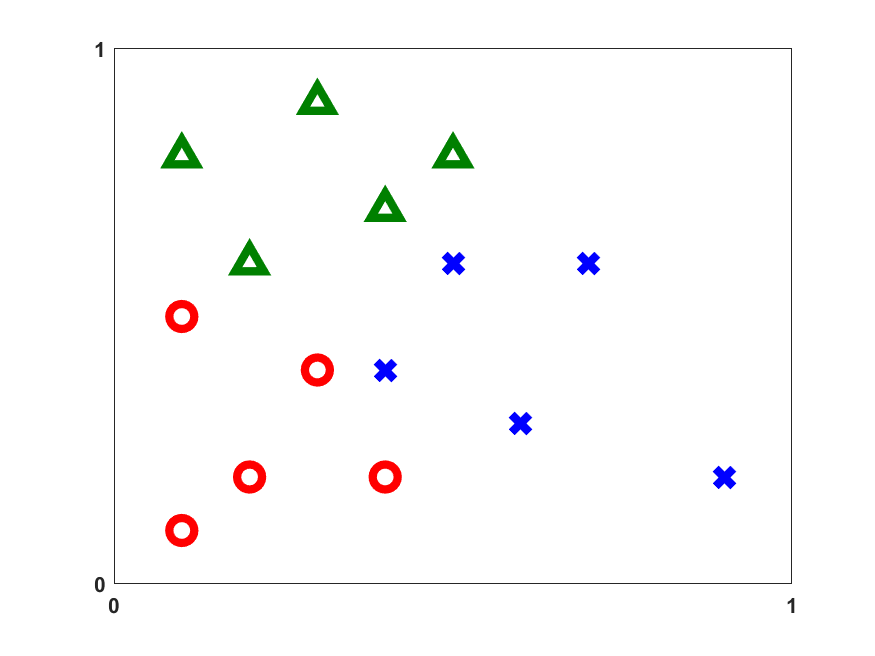
\includegraphics[width=0.5\textwidth]{Figuras/pic_xy.png}
    \caption{Puntos en el plano que marcan las tres categorías}
    \label{fig:Clasificacion}
\end{figure}

De este modo, nuestra red neuronal recibirá como entrada un punto del plano, y nos dirá a qué categoría pertenece, devolviendo $(1,0,0)^T$ si es de la categoría azul, $(0,1,0)^T$ si es de la categoría roja y $(0,0,1)^T$ si es de la categoría amarilla.

Lo siguiente que queremos hacer será entrenar la red neuronal, es decir, ajustar los pesos y sesgos de la red neuronal para que la salida se acerque lo máximo posible a la salida deseada. Es decir, que cuando se introduzca un punto de un tipo concreto, la salida lo asigne a la categoría adecuada. 

Designamos a $y(x)$ como la salida deseada de nuestra red neuronal, y a $F(x)$ como la salida real. Así, el error vendrá dado en función de los pesos y sesgos de la siguiente forma
\begin{equation*}
    \mathcal{L}(W^{[2]},W^{[3]},W^{[4]},b^{[2]},b^{[3]},b^{[4]})=\frac{1}{2}\sum_{x\in X}\|y(x)-F(x)\|^2,
\end{equation*}
donde $X$ es el conjunto de puntos que tenemos para entrenar la red neuronal, en nuestro caso, serán 15. Esta función es conocida como función de coste.

Así, lo que queremos hacer es minimizar esta función, es decir, encontrar los pesos que minimicen la función $\mathcal{L}$. Para ello, se utilizan algoritmos de optimización, como el descenso del gradiente. Este proceso es conocido como el entrenamiento de la red neuronal. Si se logra con éxito, la red neuronal será capaz de clasificar correctamente los puntos en el plano. En este caso concreto, al entrenar la red neuronal, se obtiene la clasificación de la Figura \ref{fig:ClasificacionFinal}, en la que simplemente hemos aplicado nuestra función para cada punto del plano y lo hemos sombreado de acuerdo a la clasificación que se le ha dado. El código que se ha utilizado para entrenar la red neuronal y obtener la clasificación de la Figura \ref{fig:ClasificacionFinal} es el que se encuentra en el Anexo \ref{sec:codigo_clasificacion}

\begin{figure}
    \centering
    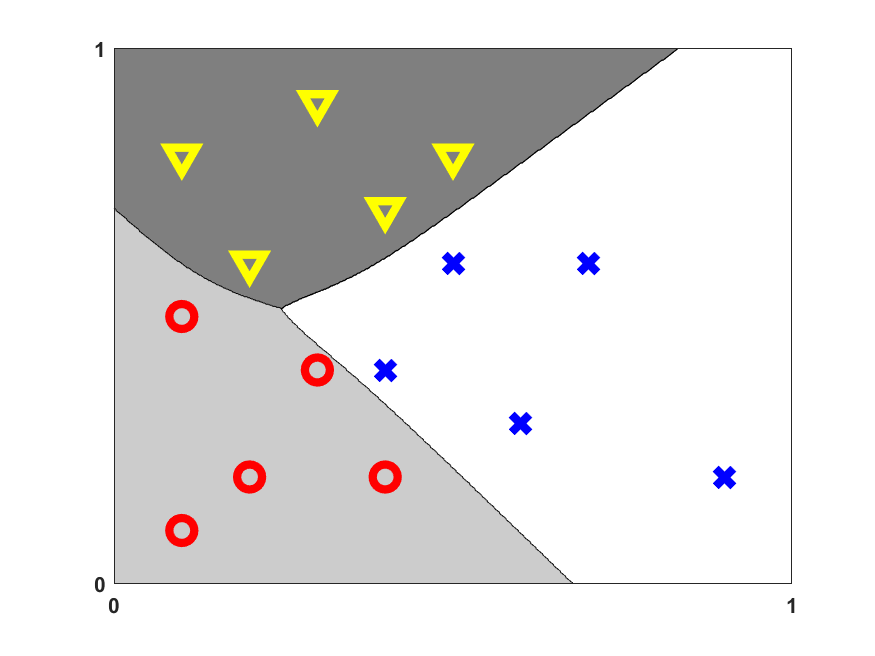
\includegraphics[width=0.5\textwidth]{Figuras/classifier_back.png}
    \caption{Puntos en el plano que marcan las tres categorías}
    \label{fig:ClasificacionFinal}
\end{figure}

\subsection{Comentarios sobre la función sigmoide}\label{subsec:Sigmoide}
Como hemos visto con el ejemplo anterior, las redes neuronales se pueden utilizar para generar funciones. A su vez, estas funciones se utilizan para resolver problemas de forma aproximada. En el ejemplo de la Figura \ref{fig:ClasificacionFinal}, la función red neuronal clasifica cualquier parte del plano en una de las tres categorías sombreadas a partir del entrenamiento. Dicho entrenamiento fija los valores de los pesos y sesgos, y por tanto define la función red neuronal (en el ejemplo define la función \eqref{eq:RedNeuronal}).

Como las redes neuronales se utilizan para aproximar problemas de tipos muy distintos, una de las características deseables es que sean  capaces de aproximar el conjunto de funciones "mayor posible".

Para poder lograr este objetivo, se necesitan las funciones de activación. Como ejercicio, supongamos que en nuestra ecuación \eqref{eq:RedNeuronal} en lugar de utilizar la función sigmoide, no utilizamos ninguna función de activación, es decir, que nuestra red neuronal es simplemente una composición de funciones lineales. En este caso, nuestra red tendría la siguiente forma

\begin{equation*}
    F(x)=W^{[4]}(W^{[3]}(W^{[2]}x+b^{[2]})+b^{[3]})+b^{[4]}\in\mathbb{R}^3.
\end{equation*}

Claramente, una función lineal definida de forma global puede estar muy lejos de aproximar bien funciones generales. De este modo, parece por tanto razonable utilizar funciones de activación no lineales. La función sigmoide es una de las más utilizadas, pero existen otras como la función tangente hiperbólica o la función ReLU. La función sigmoide se define como:
\begin{equation*}
    \sigma(x)=\frac{1}{1+e^{-x}}.
\end{equation*}

Esta función tiene la ventaja de que su derivada es fácil de calcular, y es precisamente esta derivada la que se utiliza en el algoritmo de entrenamiento de la red neuronal.

Un resultado relevante para justificar el uso de funciones de activación no lineales es el siguiente propuesto por Pinkus \cite[Theorem 3.1]{pinkus1999approximation}. Este resultado es para redes neuronales de una sola capa.

\begin{teor}[Pinkus]
    Sea $\sigma\in C(\mathbb{R})$ y sea $\mathcal{M}(\sigma) = \text{span}\{\sigma(w\cdot x + b): b \in \mathbb{R}, w \in \mathbb{R}^n\}$, se cumple que:
    
    Para cualquier $f \in C(\mathbb{R}^n)$, cualquier conjunto compacto $K\in \mathbb{R}^n$ y cualquier $\epsilon > 0$, existe una función $g\in \mathcal{M}(\sigma)$ tal que $\max_{x\in K}|f(x)-g(x)|<\epsilon$ si y solo si $\sigma$ no es una función polinómica.
\end{teor}
De forma más intuitiva, cualquier función $f \in C(\mathbb{R}^n)$, se puede aproximar tan bien como se quiera con una red neuronal de una sola capa si y solo si la función de activación no es polinómica.

Este resultado nos aporta una intuición de por qué las funciones de activación no lineales son necesarias para aproximar funciones de forma general pues, de no ser funciones no lineales, habría muchas funciones que no podríamos aproximar. 

\section{Conceptos preliminares sobre las ecuaciones en derivadas parciales} \label{sec:EDPs}

En este trabajo nos vamos a centrar en las ecuaciones en derivadas parciales elípticas, definidas con la siguiente forma general.

\begin{mdframed}
\begin{defin}\label{def:EDP_eliptica}
    Dado un conjunto $\Omega$, acotado y abierto en $\mathbb{R}^n$, decimos que una ecuación en derivadas parciales es elíptica si es de la siguiente forma:
    \begin{equation}\label{eq:EDP_eliptica}
        -\sum_{i,j=1}^{n} \frac{\partial}{\partial x_j}\left( a_{ij}(x)\frac{\partial u}{\partial x_i}\right) + \sum_{i=1}^{n} b_i(x)\frac{\partial u}{\partial x_i} + c(x)u = f(x), \qquad x\in\Omega.
    \end{equation}
    Donde los coeficientes $a_{ij}(x)$, $b_i(x)$, $c(x)$ y $f$ son funciones que satisfacen las siguientes condiciones
    \begin{align}
        a_{ij} \in C^1(\overline{\Omega}),& \qquad i,j = 1, \dots ,n \label{eq:condiciones_EDP_eliptica_a} \\
        b_i, c \in C(\overline{\Omega}),& \qquad i = 1, \dots ,n \\
        c \in C(\overline{\Omega}),& \\
        f\in C(\overline{\Omega})&\label{eq:condiciones_EDP_eliptica_f}
    \end{align}
    y además cumple la condición de elipticidad uniforme, es decir
    \begin{equation}\label{eq:condiciones_EDP_eliptica_elipticidad_uniforme}
        \sum_{i,j=1}^n a_{ij}(x) \xi_i \xi_j \geq \tilde{c} \sum_{i=1}^n \xi_i^2, \quad \forall \xi = (\xi_1, \ldots, \xi_n) \in \mathbb{R}^n, \quad x \in \overline{\Omega},
    \end{equation}
    donde $\tilde{c}$ es una constante positiva independiente de $x$ y $\xi$.
\end{defin}
\end{mdframed}

Concretamente, a lo largo del trabajo, nos centraremos en problemas de condición de frontera de Dirichlet, es decir, problemas en los que se cumple que
\begin{equation}
    u(x) = g(x), \qquad \forall x\in\partial\Omega.
\end{equation}

En la formulación que hemos dado de las ecuaciones en derivadas parciales elípticas, nos estábamos refiriendo a su formulación en forma fuerte. No obstante, en muchos casos, no es posible encontrar una solución en forma fuerte, es decir, una función que cumpla las condiciones de frontera. En estos casos, se recurre a la  formulación débil de la ecuación, que permite encontrar una solución en un espacio de funciones más amplio. Para entender la formulación débil de una ecuación en derivadas parciales, es necesario introducir el concepto de derivada débil.

\begin{mdframed}
    \begin{defin}
        Supongamos que $u$ es localmente integrable en $\Omega$. Supongamos que también existe una función $w_\alpha$, localmente integrable en $\Omega$, tal que
        \begin{equation*}
            \int_\Omega w_\alpha(x)v(x) \, dx = (-1)^{|\alpha|} \int_\Omega u(x)D^\alpha v(x) \, dx, \qquad \forall v \in C_0^\infty(\Omega),
        \end{equation*}
        entonces decimos que $w_\alpha$ es la derivada débil de $u$ de orden $|\alpha| = \alpha_1 + \cdots + \alpha_n$ y escribimos $w_\alpha = D^\alpha u$. Cuando existe la derivada débil, es única. En lo sucesivo utilizaremos la misma notación para las derivadas débiles y fuertes.
    \end{defin}
\end{mdframed}
También es necesario definir el espacio de Sobolev $H^1(\Omega)$.
\begin{mdframed}
\begin{defin}
    Sea $\Omega$ un conjunto abierto de $\mathbb{R}^n$. Definimos el espacio de Sobolev $H^1(\Omega)$ como el conjunto de funciones en el siguiente conjunto
    \begin{equation}
        H^1(\Omega)=\{u\in L^2(\Omega): \frac{\partial u}{\partial x_i}\in L^2(\Omega), \, i=1,\dots,n\}.
    \end{equation}
    En este espacio, se define la siguiente norma
    \begin{equation}
        \|u\|_{H^1(\Omega)}=\left(\|u\|^2_{L^2(\Omega)} + \sum_{i=1}^{n}\left\|\frac{\partial u}{\partial x_i}\right\|^2_{L^2(\Omega)}\right)^{1/2}.
    \end{equation}
    En ambas definiciones las derivadas parciales se entienden en sentido débil.
\end{defin}
\end{mdframed}
    
Definimos demás el espacio $H_0^1(\Omega)$. Este espacio es el cierre de las funciones de $C_0^\infty(\Omega)$ en la norma de $H^1(\Omega)$. Es decir, $H_0^1(\Omega)$ es el conjunto de funciones $u\in H^1(\Omega)$ que se obtienen como límite en $H^1(\Omega)$ de una serie de funciones $\{u_m\}_{m=1}^\infty$ todas ellas en $C_0^\infty(\Omega)$. Si $\partial\Omega$ es suficientemente regular, $H_0^1(\Omega)$ es el siguiente conjunto:
\begin{equation}
    H_0^1(\Omega)=\{u\in H^1(\Omega): u=0 \text{ en } \partial\Omega\}.
\end{equation}

Con esto, podemos definir la solución débil de una ecuación en derivadas parciales elíptica de la siguiente forma.
\begin{mdframed}
\begin{defin}\label{def:SolucionDebil}
    Dadas las funciones $a_{ij} \in L^\infty(\Omega), \, i,j = 1,\dots, n, \, b_i \in L^\infty(\Omega), \\i= 1, \dots, n, \, c\in L^\infty(\Omega)$, y la función $f\in L^2(\Omega)$. Decimos que la función $u\in H^1_0(\Omega)$ es una solución débil de la ecuación \eqref{eq:EDP_eliptica} con condición de contorno Dirichlet homogénea, es decir, $g(x)=0$ si se cumple que, 
    \begin{equation}\label{eq:SolucionDebil}
        \begin{aligned}
            \sum_{i,j=1}^{n} \int_\Omega a_{ij}(x) \frac{\partial u}{\partial x_i} \frac{\partial \varphi}{\partial x_j}\,dx + \sum_{i=1}^{n} \int_\Omega b_i(x)\frac{\partial u}{\partial x_i} \varphi \,dx  \\+ \int_\Omega c(x)u \varphi \,dx = \int_\Omega f(x)\varphi(x) dx, \qquad \forall \varphi \in H^1_0(\Omega),
        \end{aligned}
    \end{equation}
    donde todas las derivadas parciales en la ecuación \eqref{eq:SolucionDebil} se entienden en sentido débil.
\end{defin}
\end{mdframed}

Si $u $ es una solución clásica de \eqref{eq:EDP_eliptica}, entonces también es una solución débil de \eqref{eq:SolucionDebil}. Sin embargo, lo contrario no es cierto: una solución débil puede no ser lo suficientemente regular para ser una solución clásica. En particular, se demostrará que la ecuación \eqref{eq:EDP_eliptica} tiene una solución débil única $u \in H^1_0(\Omega) $. Para simplificar la notación, se introduce la forma bilineal:
\begin{equation}
    \begin{aligned}
        a(u,\varphi) &= \sum_{i,j=1}^{n} \int_\Omega a_{ij}(x) \frac{\partial u}{\partial x_i} \frac{\partial \varphi}{\partial x_j}\,dx + \sum_{i=1}^{n} \int_\Omega b_i(x)\frac{\partial u}{\partial x_i} \varphi \,dx  \\ &+ \int_\Omega c(x)u \varphi \,dx,
    \end{aligned}
\end{equation}
y el funcional lineal,
\begin{equation}
    l(\varphi) = \int_\Omega f(x)\varphi(x) dx.
\end{equation}
De este modo, nuestro problema elíptico en forma débil se puede expresar de la siguiente manera: Encontrar $u\in H^1_0(\Omega)$ tal que
\begin{equation}\label{eq:ProblemaDebilFormaBilineal}
    a(u,\varphi) = l(\varphi) \quad \forall \varphi\in H^1_0(\Omega).
\end{equation}

Para demostrar la existencia y unicidad de solución débil, se aplica el teorema de Lax-Milgram. 

\begin{teor}[Lax-Milgram]
    Sea $V$ un espacio de Hilbert con una norma asociada $\|\cdot\|_V$, y sea $a:V\times V\rightarrow\mathbb{R}$ una forma bilineal y $l:V\rightarrow\mathbb{R}$ un funcional lineal. Si se cumplen las siguientes condiciones
    \begin{itemize}
        \item[(a)] $\exists c_0 > 0 \quad \forall v \in V \quad a(v,v) \geq c_0\|v\|^2$,
        \item[(b)] $\exists c_1 > 0 \quad \forall v, w \in V \quad |a(w,v)| \leq c_1\|w\|\|v\|$,
    \end{itemize}
    y sea $l(\cdot)$ un funcional lineal en $V$ tal que:
    \begin{itemize}
        \item[(c)] $\exists c_2 > 0 \quad \forall v \in V \quad |l(v)| \leq c_2\|v\|$.
    \end{itemize}
    entonces, existe una única solución débil $u\in V$ tal que
    \begin{equation*}
        a(u,v) = l(v) \quad \forall v\in V.
    \end{equation*}
\end{teor}
Con este teorema se puede demostrar que una ecuación elíptica con condiciones de contorno Dirichlet homogéneas tiene solución única en $H^1_0(\Omega)$. Para ello se puede aplicar el teorema de Lax-Milgram en el espacio $V=H^1_0(\Omega)$ con la norma $\|\cdot\|_{H^1(\Omega)}$ y las formas bilineal y lineal $a$ y $l$ definidas anteriormente. Para que se cumplan las condiciones $(a,b,c)$ del teorema, además de la condición de elipticidad uniforme es necesario requerir que
\begin{equation}\label{eq:condiciones_LaxMilgram_extra}
    c(x) - \frac{1}{2} \sum_{i=1}^n \frac{\partial b_i}{\partial x_i} \geq 0, \quad x \in \overline{\Omega}.
\end{equation}

De esta manera, se demuestran las condiciones (a), (b) y (c) del teorema de Lax-Milgram como sigue.
\begin{dem}
    Empezamos por la condición (c).
    \begin{itemize}
        \item[(c)] La aplicación $v \mapsto l(v)$ es lineal: de hecho, para cualesquiera $\alpha, \beta \in \mathbb{R}$, 
        \begin{align*}
            l(\alpha v_1 + \beta v_2) &= \int_{\Omega} f(x)(\alpha v_1(x) + \beta v_2(x)) \, dx \\
            &= \alpha \int_{\Omega} f(x)v_1(x) \, dx + \beta \int_{\Omega} f(x)v_2(x) \, dx \\
            &= \alpha l(v_1) + \beta l(v_2), \quad v_1, v_2 \in H_0^1(\Omega).
        \end{align*}
        Por lo tanto, $l(\cdot)$ es una funcional lineal en $H_0^1(\Omega)$. Además, por la desigualdad de Cauchy-Schwarz,
        \begin{align*}
            |l(v)| &= \left| \int_{\Omega} f(x)v(x) \, dx \right| \leq \left(\int_{\Omega} |f(x)|^2 \, dx \right)^{1/2} \left(\int_{\Omega} |v(x)|^2 \, dx \right)^{1/2} \\
            &= \|f\|_{L^2(\Omega)} \|v\|_{L^2(\Omega)} \leq \|f\|_{L^2(\Omega)} \|v\|_{H^1(\Omega)},
        \end{align*}
        para todo $v \in H_0^1(\Omega)$, donde hemos usado la desigualdad obvia $\|v\|_{L^2(\Omega)} \leq \|v\|_{H^1(\Omega)}$. Tomando $c_2 = \|f\|_{L^2(\Omega)}$, obtenemos la cota requerida.
        \item [(b)] A continuación, verificamos (b). Para cualquier $w \in H_0^1(\Omega)$, la aplicación $v \mapsto a(v, w)$ es lineal. De manera similar, para cualquier $v \in H_0^1(\Omega)$, la aplicación $w \mapsto a(v, w)$ es lineal. Por lo tanto, $a(\cdot, \cdot)$ es una funcional bilineal en $H_0^1(\Omega) \times H_0^1(\Omega)$. Aplicando la desigualdad de Cauchy-Schwarz, deducimos que
        \begin{align*}
            |a(w, v)| \leq & \sum_{i, j = 1}^n \max_{x \in \overline{\Omega}} |a_{ij}(x)|\left| \int_{\Omega}  \frac{\partial w}{\partial x_i} \frac{\partial v}{\partial x_j} dx \right|  \\
            &+ \sum_{i = 1}^n \max_{x \in \overline{\Omega}} |b_i(x)| \left|  \int_{\Omega} \frac{\partial w}{\partial x_i} v dx \right| \\
            &+ \max_{x \in \overline{\Omega}} |c(x)| \left| \int_{\Omega}  w(x)v(x) dx \right|  \\
            &\leq \hat{c} \Bigg\{
            \left( \sum_{i,j=1}^n \int_\Omega \left| \frac{\partial w}{\partial x_i} \right|^2 dx \right)^{1/2}
            \left( \int_\Omega \left| \frac{\partial v}{\partial x_j} \right|^2 dx \right)^{1/2}\\
            &+ \sum_{i=1}^n \left( \int_\Omega \left| \frac{\partial w}{\partial x_i} \right|^2 dx \right)^{1/2}
            \left( \int_\Omega |v|^2 dx \right)^{1/2} \\
            &+ \left( \int_\Omega |w|^2 dx \right)^{1/2}
            \left( \int_\Omega |v|^2 dx \right)^{1/2}
            \Bigg\}\\
            &\leq \hat{c} \Bigg\{
            \left( \int_\Omega |w|^2 dx \right)^{1/2}
            + \sum_{i=1}^n \left( \int_\Omega \left| \frac{\partial w}{\partial x_i} \right|^2 dx \right)^{1/2}
            \Bigg\} \\
            &\times
            \Bigg\{
            \left( \int_\Omega |v|^2 dx \right)^{1/2}
            + \sum_{j=1}^n \left( \int_\Omega \left| \frac{\partial v}{\partial x_j} \right|^2 dx \right)^{1/2}
            \Bigg\}.
        \end{align*}
        donde
        \begin{align*}
            \hat{c} = \max \Bigg\{ \max_{1 \leq i,j \leq n} \max_{x \in \overline{\Omega}} |a_{ij}(x)|, \max_{1 \leq i \leq n} \max_{x \in \overline{\Omega}} |b_i(x)|, \max_{x \in \overline{\Omega}} |c(x)| \Bigg\}.
        \end{align*}

        Si acotamos aún más el lado derecho de la última desigualdad, deducimos que
        \begin{align*}
            |a(w, v)| \leq (n+1)\hat{c} \Bigg\{ \left(\int_{\Omega} |w|^2 dx + \sum_{i=1}^n \int_{\Omega} \left| \frac{\partial w}{\partial x_i} \right|^2 dx \right)^{1/2} \\
            \times \left(\int_{\Omega} |v|^2 dx + \sum_{j=1}^n \int_{\Omega} \left| \frac{\partial v}{\partial x_j} \right|^2 dx \right)^{1/2} \Bigg\},
        \end{align*}
        por lo que, tomando $c_1 = (n+1)\hat{c}$, obtenemos la desigualdad de (b).
        \item[(a)] Por último, demostramos la condición (a). Aquí utilizaremos la condición extra requerida en \eqref{eq:condiciones_LaxMilgram_extra} y la condición de elipticidad uniforme \eqref{eq:condiciones_EDP_eliptica_elipticidad_uniforme}. Usando  \eqref{eq:condiciones_EDP_eliptica_elipticidad_uniforme} y la desigualdad de Cauchy-Schwarz, 
        
        \begin{equation*}
        a(v, v) \geq \tilde{c} \sum_{i=1}^n \int_\Omega \left| \frac{\partial v}{\partial x_i} \right|^2 dx
        + \sum_{i=1}^n \int_\Omega b_i(x) \frac{1}{2} \frac{\partial}{\partial x_i} (v^2) dx
        + \int_\Omega c(x) |v|^2 dx,
        \end{equation*}

        donde escribimos \(\frac{\partial v}{\partial x_i} \cdot v\) como \(\frac{1}{2} \frac{\partial}{\partial x_i}(v^2)\). Integrando por partes el segundo término en el lado derecho, obtenemos

        \begin{equation*}
        a(v, v) \geq \tilde{c} \sum_{i=1}^n \int_\Omega \left| \frac{\partial v}{\partial x_i} \right|^2 dx
        + \int_\Omega \left( c(x) - \frac{1}{2} \sum_{i=1}^n \frac{\partial b_i}{\partial x_i} \right) |v|^2 dx.
        \end{equation*}

        Asumiendo que se cumple \eqref{eq:condiciones_LaxMilgram_extra} llegamos a la desigualdad 
        \begin{align}\label{eq:resultado_aplicar_condicion_a}
        a(v, v) \geq  \tilde{c} \sum_{i=1}^{n} \int_{\Omega} \left| \frac{\partial v}{\partial x_i} \right|^2 dx.
        \end{align}
        Mediante la desigualdad de Poincaré-Friedrichs, el lado derecho puede acotarse aún más para obtener
        \begin{align}\label{eq:desigualdad_Poincaré_Friedrichs_demo_a}
        a(v, v) \geq \frac{\tilde{c}}{c_{\star}} \int_{\Omega} |v|^2 dx.
        \end{align}
        Juntando \eqref{eq:resultado_aplicar_condicion_a} y \eqref{eq:desigualdad_Poincaré_Friedrichs_demo_a}, obtenemos
        \begin{equation}\label{eq:desigualdad_final_demo_a}
        a(v, v) \geq c_0 \left( \int_{\Omega} |v|^2 dx + \sum_{i=1}^{n} \int_{\Omega} \left| \frac{\partial v}{\partial x_i} \right|^2 dx \right),
        \end{equation}
        donde $c_0 = \tilde{c}/(1 + c_{\star})$, y por queda demostrado (a).
    \end{itemize}
    Se comprueban así las condiciones (a), (b) y (c) del teorema de Lax-Milgram y concluimos que existe una única solución débil en $H^1_0(\Omega)$ para la ecuación \eqref{eq:ProblemaDebilFormaBilineal}.
\end{dem}

\section{Métodos numéricos tradicionales: el método de los elementos finitos}\label{sc:FEM}

El método de los elementos finitos (FEM por su siglas en inglés) es una técnica numérica para resolver ecuaciones en derivadas parciales. Este método es ampliamente utilizado en ingeniería y ciencias aplicadas porque permite aproximar soluciones en dominios complejos.

Para un problema elíptico con condiciones de contorno Dirichlet homogéneas, se parte de la ecuación en su formulación débil. Como hemos visto en el apartado anterior, este problema se puede formular de forma simplificada como encontrar $u\in H_0^1(\Omega)$ tal que
\begin{equation*}
    a(u,\varphi) = l(\varphi) \quad \forall \varphi\in  H_0^1(\Omega).
\end{equation*}

Por lo visto en la Sección \ref{sec:EDPs}, esta ecuación tiene solución única en $H_0^1(\Omega)$ si se cumple la condición \eqref{eq:condiciones_LaxMilgram_extra}. De este modo, para que la formulación del problema sea válida, asumiremos que se cumple esta condición.

Lo siguiente que se hace es dividir el dominio $\Omega$ en un conjunto de subdominios más pequeños, llamados elementos finitos. Por ejemplo, si estamos trabajando con un problema en un dominio unidimensional, con $\Omega =(0,1)$, dividimos $\overline{\Omega} = [0,1]$ en $N$ subintervalos $[x_i,x_{i+1}], \, i = 1, \dots, N-1$, con $x_i = ih$, obteniendo la división de la Figura \ref{fig:DivisionOmega}.

\begin{figure}
    \centering
    \begin{tikzpicture}
        \draw[thick] (0,0) -- (12,0); % Adjusted length of the line
        \foreach \x in {0,2,4,6,8,10,12} % Adjusted positions of the ticks
        \draw (\x cm,3pt) -- (\x cm,-3pt);
        \draw (0,0) node[below=3pt] {$x_0 = 0$};
        \draw (2,0) node[below=3pt] {$x_1$};
        \draw (4,0) node[below=3pt] {$x_2$};
        \draw (6,0) node[below=3pt] {$x_3$};
        \draw (8,0) node[below=3pt] {$\dots$};
        \draw (10,0) node[below=3pt] {$x_{N-1}$};
        \draw (12,0) node[below=3pt] {$x_{N}=1$};
    \end{tikzpicture}
    \caption{División de $\Omega = (0,1)$ en $N$ elementos finitos}
    \label{fig:DivisionOmega}
\end{figure}

A esta subdivision, se le asocia una base de polinomios a trozos. Reemplazando así el subespacio de funciones que habíamos llamado $H_0^1(\Omega)$ por un subespacio de dimensión finita $V_h$ formado por polinomios a trozos  de grado fijo. Siguiendo nuestro ejemplo de antes, la base de polinomios que vamos a utilizar será la de los polinomios como los vistos en la Figura \ref{fig:BasePolinomios}, definidos de la siguiente forma.
\begin{equation*}
    \phi_i(x) = \begin{cases}
        \frac{x-x_{i-1}}{x_i-x_{i-1}}, & \text{si } x\in[x_{i-1},x_i],\\
        \frac{x_{i+1}-x}{x_{i+1}-x_i}, & \text{si } x\in[x_i,x_{i+1}],\\
        0, & \text{en otro caso}.
    \end{cases} 
\end{equation*}

\begin{figure}
    \centering
    \begin{tikzpicture}[scale=0.5]
        \draw[thick] (0,0) -- (12,0); % Adjusted length of the line
        \draw (6 cm,100pt) -- (6 cm,-5pt);
        \draw (1 cm,5pt) -- (1 cm,-5pt);
        \draw (11 cm,5pt) -- (11 cm,-5pt);
        \draw[thick] (1,0) -- (6,100pt) -- (11,0);
        \draw (1,0) node[below=3pt] {$x_{i-1}$};
        \draw (6,0) node[below=3pt] {$x_i$};
        \draw (11,0) node[below=3pt] {$x_{i+1}$};
    \end{tikzpicture}
    \caption{Polinomio $\phi_i$}
    \label{fig:BasePolinomios}
\end{figure}

En este ejemplo, nuestro espacio de funciones será $V_h = \text{span}\{\phi_1,\dots,\phi_{N-1}\}$, donde $N$ es el número de elementos finitos en los que hemos dividido el dominio. Con esta definición es claro que todos los $\phi_i\in H_0^1(\Omega)$ pues son funciones derivables en sentido débil que valen $0$ en la frontera de $\Omega =(0,1)$. De este modo, al buscar soluciones en este nuevo espacio de funciones, nuestra ecuación diferencial elíptica se convertiría en encontrar $u_h\in V_h$ tal que
\begin{equation*}
    a(u_h,v_h) = l(v_h) \quad \forall v_h\in V_h.
\end{equation*}
Nótese que las condiciones de contorno van implícitas en la definición de $V_h$ pues todos los $\phi_i\in H_0^1(\Omega)$. 

Con todo, de forma intuitiva, lo que se hace es que en vez de buscar una solución en un espacio de funciones de dimensión infinita, como es $H_0^1(\Omega)$, se busca una solución en un espacio de funciones de dimensión finita, como es $V_h$. Para poder hacer eso, que nos simplifica mucho el problema, lo que hemos hecho es que nuestro dominio, lo hemos dividido en subdominios más pequeños a partir de los cuales hemos construido nuestro nuevo espacio de funciones. 

Ahora, encontrar una solución se convierte en encontrar los coeficientes en la base de polinomios a trozos, es decir, los $U_i$ en la siguiente ecuación
\begin{equation}
    u_h = \sum_{i=1}^{N-1} U_i\phi_i.
\end{equation}
Por tanto, resolver la ecuación diferencial se convierte en encontrar $U=(U_1,\dots, U_{N-1}) \in \mathbb{R}^{N-1}$ que cumplen:
\begin{equation}
    \sum_{i=1}^{N-1} a\left( \phi_i,\phi_j\right)U_i = l(\phi_j) \quad \forall j = 1,\dots,N-1.
\end{equation}

Esto se traduce en un sistema lineal de la forma $AU = b$, donde $A$ es la matriz de rigidez (con entradas $A_{ij}=a\left( \phi_i,\phi_j\right)$), y $b$ es el vector de términos fuente (con entradas $b_j = l(\phi_j)$). A este nuevo sistema lineal se le pueden aplicar métodos numéricos tradicionales para resolverlo, como la factorización LU, encontrando así los coeficientes $U$ que nos dan $u_h$, la aproximación de $u$.

Este proceso se puede generalizar a problemas en más dimensiones, donde se dividen los dominios en elementos finitos de mayor dimensión, y se construye una base de polinomios a trozos en cada uno de estos elementos. Por ejemplo, en dos dimensiones, un elemento finito sería un triángulo, y la base de polinomios a trozos sería una base de funciones que valen que valen $1$ en uno de los nodes de la partición, $0$ en el resto de nodos y además son lineales en cada uno de los triángulos.

\begin{mdframed}  
\begin{exmp}
    Veamos ahora un ejemplo concreto de la aplicación del FEM a través de la ecuación de Poisson en dos dimensiones. El objetivo es encontrar un campo escalar $ u $ sobre un dominio $\Omega \subset \mathbb{R}^2$ que satisfaga:
    \begin{equation}
    \begin{aligned}
    - \Delta u &= f \quad \text{en} \ \Omega, \\
    u &= 0 \quad \text{en} \ \partial\Omega, \\
    \end{aligned}
    \end{equation}
    donde $ f $ es un término fuente y la condición de contorno es de Dirichlet homogénea. Para encontrar una solución, construimos la forma débil de la ecuación. Para ello, tomamos $v\in H_0^1(\Omega)$ y multiplicamos ambos lados por $v$ e integramos sobre $\Omega$.
    \begin{equation*}
        -\int_{\Omega} (\Delta u) v \, dx = \int_{\Omega} f v \, dx.
    \end{equation*}
    Utilizando la identidad $div(v\nabla u) = (\nabla u)(\nabla v) + v \Delta u$ obtenemos:
    \begin{equation*}
    \int_{\Omega} \nabla u \nabla v - \int_{\Omega} div(v \nabla u) = \int_{\Omega} f v
    \end{equation*}
    Por el teorema de Green, podemos escribir (si \(\partial \Omega\) es suficientemente regular):
    \begin{equation*}
    \int_{\Omega} \nabla u \nabla v - \int_{\partial \Omega} (v \nabla u) \cdot \mathbf{n} \, dS = \int_{\Omega} f v
    \end{equation*}
    Finalmente, dado que \(v = 0\) en \(\partial \Omega\), concluimos:
    \begin{equation*}
    \int_{\Omega} \nabla u \nabla v = \int_{\Omega} f v
    \end{equation*}
    La forma fuerte del problema se convierte en: 
    \begin{equation}\label{eq:forma_debil_poisson}
    a(u, v) = l(v) \quad \forall \ v \in H_0^1(\Omega),
    \end{equation}
    donde:
    \begin{itemize}
        \item $ a(u, v) = \int_{\Omega} \nabla u \cdot \nabla v \, \text{d}x $
        \item $ l(v) = \int_{\Omega} f v \, dx $
    \end{itemize}
    Para aplicar el FEM, nos interesa encontrar una solución aproximada en un espacio de funciones de dimensión finita. Para ello, dividimos el dominio $\Omega$ en un conjunto de elementos finitos y construimos una base de polinomios a trozos en cada uno de estos elementos. 
    
    Antes de seguir avanzando, para este ejemplo específico, tomaremos un dominio cuadrado $\Omega = (0,1)^2$ y $f(x, y) = 1$. Bajo estas condiciones sabemos que existe una solución única en $H_0^1(\Omega)$ para el problema \eqref{eq:forma_debil_poisson}.

    A continuación, usamos el paquete de Python Scipy para construir la malla de elementos finitos y la base de polinomios necesarias para resolver el problema (código comentado en el Anexo \ref{sec:codigo_fem_cuadrado}). El resultado obtenido se muestra en la Figura \ref{fig:poisson}, donde la malla de elementos finitos está compuesta por 50 nodos en cada lado.
    \begin{figure}[H] 
        \centering
        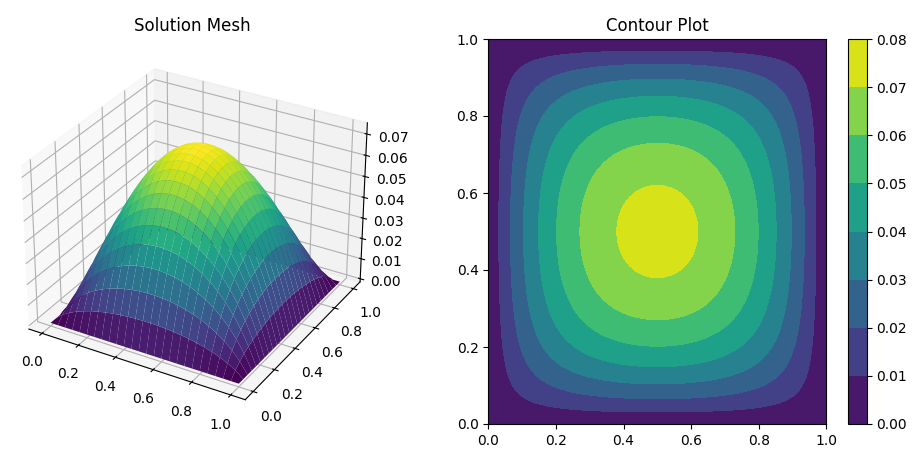
\includegraphics[width=1\textwidth]{Figuras/FEMSquare.png}
        \caption{Solución de la ecuación de Poisson}
        \label{fig:poisson}
    \end{figure}
\end{exmp}
\end{mdframed}

\chapter{Aproximación de EDPs mediante redes neuronales}\label{chap2}

\section{PINNs: Physics-Informed Neural Networks}\label{sec:PINN}
\subsection{Introducción}
Las PINNs, o Physics-Informed Neural Networks, son una técnica que combina la resolución de ecuaciones en derivadas parciales con redes neuronales. La idea es que, en vez de resolver la ecuación diferencial directamente o con métodos numéricos tradicionales, se entrena una red neuronal para que aproxime la solución de la ecuación. 

Como habíamos comentado en la Sección \ref{sec:RedesNeuronales}, las redes neuronales son capaces de aproximar cualquier función, por lo que, en teoría, pueden aproximar cualquier solución de una ecuación diferencial. De este modo, las PINNs van a aprovechar esto, definiendo la aproximación de nuestra solución ${u}$, como la salida de la función red neuronal $\hat{u}(x;\mathbf{\theta})$,  donde $\theta$ hace referencia a los pesos y sesgos vistos en la Sección \ref{sec:RedesNeuronales}. Así, la función en la Figura \ref{fig:PIN} sería la aproximación de la solución de la ecuación diferencial.
\begin{figure}[htbp]
    \centering
    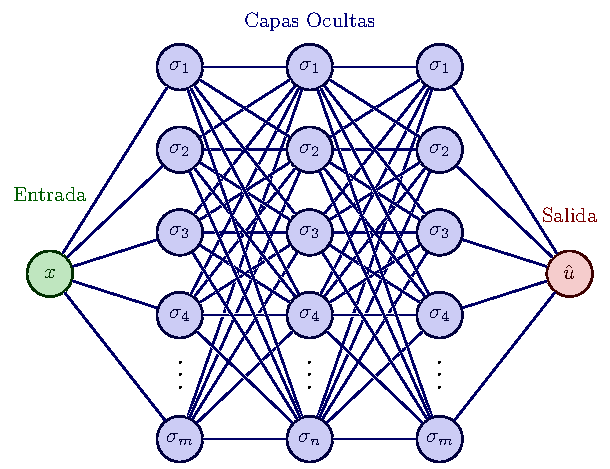
\includegraphics[scale=0.6]{Figuras/neural_network_improved.pdf}
    \caption{Esquema de una PINN}
    \label{fig:PIN}
\end{figure}

\subsection{Formulación de las PINNs}
Consideramos una EDP de la forma vista en la Sección \ref{sec:EDPs}, es decir, una EDP elíptica sujeta a condiciones de contorno Dirichlet. De modo que la ecuación a resolver es la siguiente: 
\begin{equation} 
    \begin{cases} -\sum_{i,j=1}^{n} \frac{\partial}{\partial x_j}\left( a_{ij}(\mathbf{x})\frac{\partial u}{\partial x_i}\right) + \sum_{i=1}^{n} b_i(\mathbf{x})\frac{\partial u}{\partial x_i} + c(\mathbf{x})u = f(\mathbf{x}), &\qquad \mathbf{x}\in\Omega,\\ u(\mathbf{x}) = g(\mathbf{x}), &\qquad \mathbf{x}\in\partial\Omega. 
    \end{cases} 
\end{equation} 
donde $\Omega \subset \mathbb{R}^n$ es un dominio abierto y acotado y las funciones $a_{ij}(\mathbf{x})$, $b_i(\mathbf{x})$, $c(\mathbf{x})$, $f(\mathbf{x})$ y $g(\mathbf{x})$ son conocidas. La incógnita es la función $u: \Omega \to \mathbb{R}$ que satisface la ecuación diferencial y las condiciones de contorno. Para poder construir y ajustar los pesos de una red neuronal que aproxime $u$ es esencial tener una función de coste, es decir, una función que nos indique la calidad de nuestra aproximación. 

Con las PINNs nosotros queremos encontrar una función $\hat{u}$ que minimice el residuo en $\Omega$ y que cumpla las condiciones de contorno en $\partial\Omega$. Para ello, lo que queremos es la $\hat{u}$ que haga que las siguientes expresiones sean mínimas:
\begin{align*}
    &\int_{\Omega} \left( -\sum_{i,j=1}^{n} \frac{\partial}{\partial x_j}\left( a_{ij}(\mathbf{x})\frac{\partial \hat{u}}{\partial x_i}\right) + \sum_{i=1}^{n} b_i(\mathbf{x})\frac{\partial \hat{u}}{\partial x_i} + c(\mathbf{x})\hat{u} - f(\mathbf{x}) \right)^2, \\ 
    &\int_{\partial\Omega} \left( \hat{u} (\mathbf{x}) - g(\mathbf{x})\right)^2.
\end{align*}

Para poder computar estas integrales, se utiliza una regla de cuadratura que las aproxime mediante sumas ponderadas de los valores de las funciones en un conjunto discreto de puntos. En este contexto, los puntos de evaluación se denominan puntos de colocación o collocation points. Para la primera expresión, los puntos de colocación que se usarán los denominaremos $\mathcal{T}_f$, mientras que para la segunda los denominaremos $\mathcal{T}_b$. 

Por tanto, en el caso de las PINNs, la función de coste se compone de la suma ponderada de dos términos. El primero garantiza que la red neuronal aproxime la solución de la ecuación diferencial en un conjunto discreto de puntos. El segundo asegura que dicha aproximación cumpla las condiciones de contorno de Dirichlet en otro conjunto finito de puntos.

\begin{equation} \label{eq:L_PINN}
    \mathcal{L}(\boldsymbol{\theta}; \mathcal{T}) = w_f \mathcal{L}_f(\boldsymbol{\theta}; \mathcal{T}_f) + w_b \mathcal{L}_b(\boldsymbol{\theta}; \mathcal{T}_b),
\end{equation}
donde $w_f$ y $w_b$ son pesos que se ajustan para dar más importancia a un término u otro y
\begin{equation}
    \label{eq:Lf_Lb}
    \begin{split}
        \mathcal{L}_f(\boldsymbol{\theta}; \mathcal{T}_f) &= \frac{1}{|\mathcal{T}_f|} \sum_{\mathbf{x} \in \mathcal{T}_f} | -\sum_{i,j=1}^{n} \frac{\partial}{\partial x_j}\left( a_{ij}(\mathbf{x})\frac{\partial \hat{u}}{\partial x_i}\right) \\ &+ \sum_{i=1}^{n} b_i(\mathbf{x})\frac{\partial \hat{u}}{\partial x_i} + c(\mathbf{x})\hat{u} - f(\mathbf{x}) |^2, \\ 
        \mathcal{L}_b(\boldsymbol{\theta}; \mathcal{T}_b) &= \frac{1}{|\mathcal{T}_b|} \sum_{\mathbf{x} \in \mathcal{T}_b} \left| \hat{u} (\mathbf{x}) - g(\mathbf{x})\right|^2,
    \end{split}
\end{equation}

Como hemos indicado, aquí $\mathcal{T}_f$ y $\mathcal{T}_b$ representan conjuntos de puntos en el dominio $\Omega$ y en la frontera $\partial\Omega$, respectivamente. De este modo, las funciones, $\mathcal{L}_f$ y $\mathcal{L}_b$, representan la aproximación al residuo fuerte, y la condición de contorno, por una regla de cuadratura. 



Existe mucha literatura sobre como tomar los puntos de colocación pues, al igual que en FEM la malla impacta el resultado, en las PINNs, el conjunto $\mathcal{T}$ determina como de bien nuestra red neuronal se ajusta a la solución \cite{münzer2022curriculumtrainingbasedstrategydistributingcollocation}, \cite{aikawa2024improving}, \cite{matsubara2023goodlatticetrainingphysicsinformed}, \cite{subramanian2022adaptiveselfsupervisionalgorithmsphysicsinformed}, \cite{hou2023enhancing}.  

Es importante destacar que con esta formulación, se impone que el residuo en forma fuerte de la ecuación diferencial sea cero en los puntos de colocación, lo cual, veremos más adelante que puede ser una fuente de errores. 

Dada la función de coste y la distribución de los puntos de colocación, el siguiente paso es el entrenamiento. Esto se reduce a resolver un problema de optimización: encontrar los parámetros $\theta$ que minimizan la función de coste $\mathcal{L}(\boldsymbol{\theta}; \mathcal{T})$. Para ello, es habitual emplear métodos de optimización basados en gradientes, como Adam o L-BFGS. 

Una ventaja fundamental del uso de redes neuronales en este contexto es la diferenciación automática, una técnica numérica muy potente que facilita la obtención de las derivadas de $\hat{u}$ con respecto a sus entradas de forma exacta y eficiente.
A continuación, vamos a ver dos ejemplos para ver como se aplican las PINNs a problemas concretos.

\begin{mdframed}
    \begin{exmp}
        Consideramos la ecuación elíptica unidimensional:
        \begin{equation*}
        -u_{xx} = \pi^2 \sin(\pi x), \quad x \in [-1, 1],
        \end{equation*}
        con las condiciones de contorno de Dirichlet
        \begin{equation*}
        u(-1) = 0, \quad u(1) = 0.
        \end{equation*}
        En esta ecuación la solución exacta es  conocida $ u(x) = \sin(\pi x)$. Para resolver este problema con una PINN, nos asistimos de la librería de python DeepXDE \cite{lu2021deepxde}, la cual tiene implementada la funcionalidad necesaria para entrenar una red neuronal que aproxime EDPs. Así, comenzamos definiendo el intervalo en el que se encuentra el dominio y los puntos de colocación
        
\begin{lstlisting}[language=Python]
    geom = dde.geometry.Interval(-1, 1)
\end{lstlisting}
        definimos la EDP
\begin{lstlisting}[language=Python]
    def pde(x, y):
        dy_xx = dde.grad.hessian(y, x)
        return -dy_xx - np.pi ** 2 * tf.sin(np.pi * x)
\end{lstlisting}
    indicamos las condiciones de contorno de Dirichlet
\begin{lstlisting}[language=Python]
    bc = dde.icbc.DirichletBC(geom, func, boundary)
\end{lstlisting}
y, con todo, se define el problema de EDPs
\begin{lstlisting}[language=Python]
   data = dde.data.PDE(geom, pde, bc, 16, 2, solution=func, num_test=100)
\end{lstlisting}
    Gracias a la librería DeepXDE, podemos entrenar la red neuronal con el siguiente código
\begin{lstlisting}[language=Python]
Losshistory, train_state = model.train(
    iterations=10000, callbacks=[checkpointer, movie]
)
\end{lstlisting}
    Por detrás, esta se encargará de definir la función de coste asociada, que en este caso será
    \begin{equation*} 
        \mathcal{L}(\boldsymbol{\theta}; \mathcal{T}) = w_f \mathcal{L}_f(\boldsymbol{\theta}; \mathcal{T}_f) + w_b \mathcal{L}_b(\boldsymbol{\theta}; \mathcal{T}_b),
    \end{equation*}
    donde
    \begin{align*}
        \mathcal{L}_f(\boldsymbol{\theta}; \mathcal{T}_f) &= \frac{1}{|\mathcal{T}_f|} \sum_{\mathbf{x} \in \mathcal{T}_f} | \hat{u}_{xx} +\pi^2 \sin(\pi x)|^2, \\ 
        \mathcal{L}_b(\boldsymbol{\theta}; \mathcal{T}_b) &= \frac{1}{|\mathcal{T}_b|} \sum_{\mathbf{x} \in \mathcal{T}_b} | \hat{u} (\mathbf{x})|^2,
    \end{align*}
    por los argumentos con los que se han inicializado las funciones, $\mathcal{T}_f$ serán 16 puntos aleatorios en el intervalo $[-1,1]$ y $\mathcal{T}_b = \{0,1\}$ . Con todo, el resultado de ejecutar este código será el de la Figura \ref{fig:poisson_PINN}.

    \begin{figure}[H] 
        \centering
        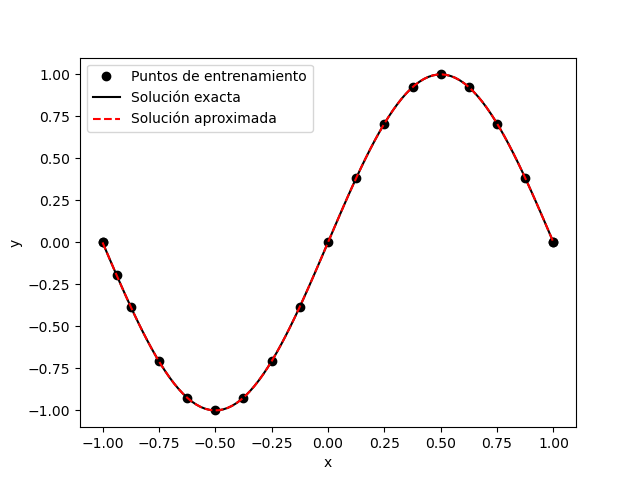
\includegraphics[width=0.6\textwidth]{Figuras/Poisson.png}
        \caption{Solución de la ecuación de Poisson}
        \label{fig:poisson_PINN}
    \end{figure}
\end{exmp}
\end{mdframed}

Aunque en este ejemplo sencillo las PINNs funcionan muy bien, estas pueden presentar errores elevados incluso en sistemas relativamente simples. A continuación, vemos uno de los ejemplos que presentan en Luo et al. en \cite{luo2023residualminimizationpdesfailure} en los que las PINNs fallan.

\begin{mdframed}
    \begin{exmp}\label{exmp:fallo}
        Consideramos la siguiente ecuación en un dominio unidimensional:
        \begin{equation}
            \left\{
            \begin{aligned}
                L u =-D_{x}(AD_{x} u) &=f\quad \text{en}\  \Omega=(-1,1), \\
                u &=0\quad \text{en}\  \partial\Omega=\{-1,1\},
            \end{aligned}
            \right.
        \end{equation}
        donde la función coeficiente $A$ y $f$ son ambas funciones continuas a trozos y se expresan como
        \begin{equation}\label{eq:1dCoeff}
            A(x)=\left\{
            \begin{aligned}
                & \tfrac{1}{2}, & & x\in (-1,0), \\
                &1, & & x\in [0,1),
            \end{aligned}
            \right.\quad 
            f(x)=\left\{
            \begin{aligned}
                & 0, & & x\in (-1,0), \\
                & -2, & & x\in [0,1).
            \end{aligned}
            \right.
        \end{equation}
        Claramente, no existe una solución fuerte. Sin embargo la solución débil $u\in H^1(-1,1)$ para esta ecuación es
        \begin{equation}\label{eq:SolTo1dEq}
            u(x)=
            \left\{
            \begin{aligned}
                & -\tfrac{2}{3}x-\tfrac{2}{3}, & & x\in (-1,0), \\
                & x^2-\tfrac{1}{3}x-\tfrac{2}{3}, & & x\in [0,1).
            \end{aligned}
            \right.
        \end{equation}
        En la serie de experimentos numéricos, utilizamos una red neuronal con la siguiente configuración $1$-$256$-$256$-$256$-$1$.  Así, la función de coste vendrá dada por la siguiente función.
        \begin{equation*} 
            \mathcal{L}(\boldsymbol{\theta}; \mathcal{T}) = w_f \mathcal{L}_f(\boldsymbol{\theta}; \mathcal{T}_f) + w_b \mathcal{L}_b(\boldsymbol{\theta}; \mathcal{T}_b),
        \end{equation*}
        donde
        \begin{align*}
            \mathcal{L}_f(\boldsymbol{\theta}; \mathcal{T}_f) &= \frac{1}{|\mathcal{T}_f|} \sum_{\mathbf{x} \in \mathcal{T}_f} |D_{x}(A(x)D_{x} w(x))+f(x)|^2, \\ 
            \mathcal{L}_b(\boldsymbol{\theta}; \mathcal{T}_b) &= \frac{1}{|\mathcal{T}_b|} \sum_{\mathbf{x} \in \mathcal{T}_b} |\hat{u} (\mathbf{x})|^2,
        \end{align*}
        En este caso, $\mathcal{T}_b=\{-1,1\}$ y $\mathcal{T}_f$ es un conjunto de 1000 puntos muestreados uniformemente en el intervalo $(-1,1)$. Es decir, $|\mathcal{T}_f|=1000$ y $|\mathcal{T}_b|=2$.

        Bajo esta configuración, obtenemos la función de red $\hat{u}(\mathbf{x};\theta)$ numéricamente a través del método PINN y la comparamos con la solución débil en la Figura \ref{fig:deviation}. 

        \begin{figure}[H] 
            \centering
            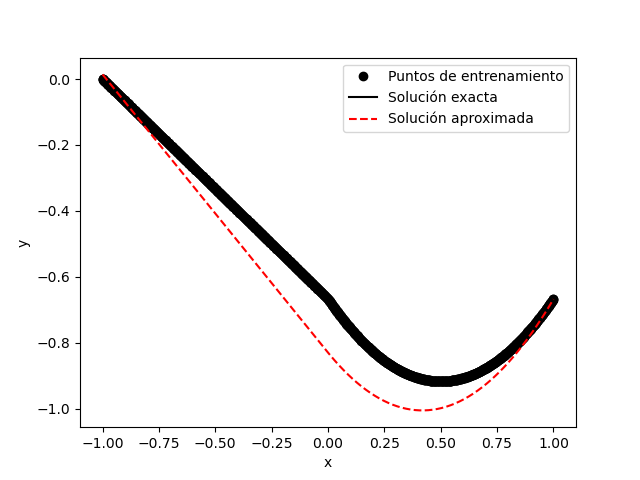
\includegraphics[width=0.6\textwidth]{Figuras/fallo_edp_pinn.png}
            \caption{Solución de la ecuación}
            \label{fig:deviation}
        \end{figure}

        Evidentemente, el método no logra obtener la solución exacta \( u \). La diferencia entre \( u \) y \( \hat{u}(\mathbf{x};\theta) \) es del mismo orden de magnitud que \( u \) en sí. En otras palabras, cuanto mayor es el valor absoluto de la solución, mayor es la desviación de la aproximación. Además, al analizar la evolución del error en las gráficas de entrenamiento y test, observamos que la diferencia entre la solución real y la aproximación, medida con la norma \( L_2 \), no disminuye con el número de iteraciones (Error relativo \( L_2 \) en el gráfico).
        \begin{figure}[H]
            \centering
            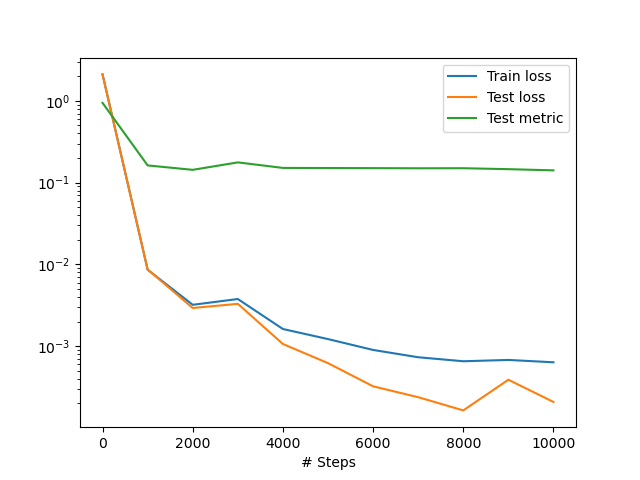
\includegraphics[width=0.6\textwidth]{Figuras/test_train_pinn_error.png}
            \caption{Error de la red neuronal}
        \end{figure}

        En esta gráfica, las curvas \textit{Error entrenamiento} y \textit{Error test} representan el error de la aproximación en los puntos de entrenamiento y test, respectivamente. Los puntos de entrenamiento corresponden al conjunto de colocación utilizado para aproximar la integral, mientras que los puntos de test pertenecen a un subconjunto del dominio donde se evalúa la aproximación. Por otro lado, el error relativo $L_2$ cuantifica la diferencia entre la solución aproximada por la red neuronal y la solución real, integrando dicha diferencia sobre el dominio $(-1,1)$. El código utilizado para este ejemplo se puede encontrar en el Anexo \ref{sec:codigo_pinns}.
    \end{exmp}
\end{mdframed}

Como hemos visto, las PINNs presentan errores significativos en ciertos problemas, lo que puede atribuirse a diversos factores. Uno de los principales desafíos de las PINNs es la falta de garantía de unicidad en la solución. A diferencia de los métodos numéricos tradicionales, las PINNs resuelven problemas de optimización no convexos, los cuales, por naturaleza, no aseguran una solución única. Esto implica que la red neuronal no tiene garantía de converger a la solución correcta y, de hecho, en muchos casos no lo hace. Es más, al igual que ocurre con otros algoritmos de inteligencia artificial, la red puede converger con la misma certeza (o error) hacia una solución incorrecta que hacia la solución real.

Otro obstáculo importante es la ausencia de una justificación teórica que determine cuáles son los hiperparámetros óptimos. Este problema añade incertidumbre al proceso de ajuste de la red, lo que complica la obtención de resultados precisos. Finalmente, otro aspecto problemático de las PINNs es que aproximan el residuo de forma fuerte. Esto significa que, si no existe una solución en el sentido fuerte (como ocurre en el ejemplo mostrado), la red neuronal no puede aproximar de forma adecuada la solución débil.

De estos problemas, los dos primeros son característicos del uso de redes neuronales, mientras que el tercero es específico del método. Con esto en mente, exploraremos un enfoque alternativo que considere la forma débil en la composición del residuo, lo que podría permitir superar esta limitación.


\section{El ``Deep Ritz Method''} \label{sec:DeepRitz}

El método ``Deep Ritz'' es una técnica numérica basada en las redes neuronales, que busca encontrar una solución a una ecuación en derivadas parciales utilizando su forma débil. La formulación de este método es más parecida al método de elementos finitos. La principal diferencia con el método de elementos finitos es el espacio donde se busca el mínimo. Nos restringimos a problemas autoadjuntos en los que la forma débil es equivalente a minimizar un funcional.



\subsection{El problema elíptico autoadjunto}\label{sec:ProblemaAutoadjunto}

El problema elíptico autoadjunto  permite caracterizar las soluciones de las EDP elípticas como el mínimo de un funcional. Esto conecta de manera lógica con el enfoque de redes neuronales para aproximar soluciones, donde la función de coste de la red neuronal se puede definir como esta función. Al minimizarla, se obtiene una solución aproximada del problema original. No obstante, esto lo veremos más adelante en detalle. De momento, consideramos una EDP de la forma vista en la Sección \ref{sec:EDPs}, es decir, una EDP elíptica sujeta a condiciones de contorno Dirichlet:
\begin{equation} 
    \begin{cases} -\sum_{i,j=1}^{n} \frac{\partial}{\partial x_j}\left( a_{ij}(\mathbf{x})\frac{\partial u}{\partial x_i}\right) + \sum_{i=1}^{n} b_i(\mathbf{x})\frac{\partial u}{\partial x_i} + c(\mathbf{x})u = f(\mathbf{x}), &\qquad \mathbf{x}\in\Omega,\\ u(\mathbf{x}) = g(\mathbf{x}), &\qquad \mathbf{x}\in\partial\Omega. 
    \end{cases} 
\end{equation} 
Se define el problema elíptico autoadjunto de la siguiente forma.
\begin{mdframed}
\begin{defin}
    Dado un conjunto $\Omega$, acotado y abierto en $\mathbb{R}^n$, decimos que una ecuación en derivadas parciales elíptica es autoadjunta, si se cumplen las siguientes condiciones de simetría en los coeficientes.
    \begin{equation}\label{eq:simetria_a}
        \begin{split}
            a_{ij} = a_{ji},\qquad &i,j = 1,\dots,n,\\
            b_i = 0, \qquad &i = 1,\dots,n,
        \end{split}
    \end{equation}
\end{defin}
\end{mdframed}
Bajo estas condiciones, nuestro problema se puede formular de la siguiente forma.
\begin{equation} \label{eq:ProblemaAutoadjuntoFuerte}
    \begin{cases}
        -\sum_{i,j=1}^{n} \frac{\partial}{\partial x_j}\left( a_{ij}(x)\frac{\partial u}{\partial x_i}\right) + c(x)u = f(x), & x\in\Omega,\\
        u(x) = 0, & x\in\partial\Omega.
    \end{cases}
\end{equation}

Por lo visto en la Sección \ref{sec:EDPs}, el problema \eqref{eq:ProblemaAutoadjuntoFuerte} se puede reescribir en forma débil de la siguiente forma: encontrar $u\in H_0^1(\Omega)$ tal que
\begin{equation}\label{eq:ProblemaAutoadjuntoDebil}
    a(u,v) = l(v) \quad \forall v\in  H_0^1(\Omega).
\end{equation}
Donde, al ser un problema autoadjunto, el funcional $a(\cdot,\cdot)$ es simétrico
\begin{equation*}
    a(u,w) = a(w,u) \quad \forall u,w\in H_0^1(\Omega).
\end{equation*}

De ahora en adelante vamos a asumir que \eqref{eq:ProblemaAutoadjuntoFuerte} cumple la condición de elipticidad uniforme y además se cumple que
\begin{equation*}
    c(x) - \frac{1}{2} \sum_{i=1}^n \frac{\partial b_i}{\partial x_i} \geq 0, \quad x \in \overline{\Omega},
\end{equation*}
por lo que, tal como se estableció en la Sección \ref{sec:EDPs}, el problema \eqref{eq:ProblemaAutoadjuntoFuerte} admite una única solución débil. La solución débil de \eqref{eq:ProblemaAutoadjuntoDebil} no solo es única, sino que también puede caracterizarse como el mínimo de un funcional. Esto es así por el siguiente resultado.



\begin{lema} \label{lema:MinimoFuncion}
    
    Definimos el funcional cuadrático $J: H_0^1(\Omega) \to \mathbb{R}$ como
    \begin{equation*}
        J(u) = \frac{1}{2}a(v,v) - l(v), \quad u\in H_0^1(\Omega),
    \end{equation*}
    de modo que las siguientes afirmaciones son equivalentes:
    \begin{enumerate}
        \item Encontrar el único $u\in H_0^1(\Omega)$ tal que $a(u,v) = l(v) \quad \forall v\in H_0^1(\Omega)$
        \item Encontrar el único $u\in H_0^1(\Omega)$ tal que $J(u) \leq J(v) \quad \forall v\in H_0^1(\Omega)$
    \end{enumerate}
\end{lema}
\begin{dem}
    Sea \( u \) la única solución débil de \eqref{eq:ProblemaAutoadjuntoDebil} en \( H_0^1(\Omega) \) y, para \( v \in H_0^1(\Omega) \), consideremos \( J(v) - J(u) \):
    \begin{align*}
    J(v) - J(u) &= \frac{1}{2} a(v,v) - l(v) - \frac{1}{2} a(u,u) + l(u) \\
    &= \frac{1}{2} a(v,v) - \frac{1}{2} a(u,u) - l(v - u) \\
    &= \frac{1}{2} a(v,v) - \frac{1}{2} a(u,u) - a(u, v - u) \\
    &= \frac{1}{2} \left[ a(v,v) - 2a(u,v) + a(u,u) \right] \\
    &= \frac{1}{2} \left[ a(v,v) - a(u,v) - a(v,u) + a(u,u) \right] \\
    &= \frac{1}{2} a(v - u, v - u).
    \end{align*}
    Por lo tanto,
    \begin{equation*}
    J(v) - J(u) = \frac{1}{2} a(v - u, v - u).
    \end{equation*}
    Debido a \eqref{eq:desigualdad_final_demo_a},
    \begin{equation*}
    a(v - u, v - u) \geq c_0 \| v - u \|_{H_0^1(\Omega)}^2,
    \end{equation*}
    donde \( c_0 \) es una constante positiva. Así,
    \begin{equation}\label{eq:J(v)-(u)}
    J(v) - J(u) \geq \frac{c_0}{2} \| v - u \|_{H_0^1(\Omega)}^2 \quad \forall v \in H_0^1(\Omega)
    \end{equation}
    y, en consecuencia,
    \begin{equation}\label{eq:J(v)geqJ(u)}
    J(v) \geq J(u) \quad \forall v \in H_0^1(\Omega)
    \end{equation}
    es decir, \( u \) minimiza \( J(\cdot) \) sobre \( H_0^1(\Omega) \).
    De hecho, \( \tilde{u} \) es el único mínimo de \( J(\cdot) \) en \( H_0^1(\Omega) \). En efecto, si \( \tilde{u} \) también minimiza \( J(\cdot) \) en \( H_0^1 (\Omega) \), entonces
    \begin{equation}\label{eq:J(v)geq(utilde)}
    J(v) \geq J(\tilde{u}) \quad \forall v \in H_0^1(\Omega).
    \end{equation}
    Tomando \( v = \tilde{u} \) en \eqref{eq:J(v)geqJ(u)} y \( v = u \) en \eqref{eq:J(v)geq(utilde)}, deducimos que
    \begin{equation*}
    J(u) = J(\tilde{u});
    \end{equation*}
    pero entonces, en virtud de \eqref{eq:J(v)-(u)},
    \begin{equation*}
    \| \tilde{u} - u \|_{H_0^1(\Omega)} = 0,
    \end{equation*}
    y, por lo tanto, \( u = \tilde{u} \). 


    Para la implicación en sentido contrario, es fácil demostrar que $J(\cdot)$ es convexa, es decir:
    \begin{equation*}
    J((1 - \theta)v + \theta w) \leq (1 - \theta)J(v) + \theta J(w) \quad \forall \theta \in [0,1], \quad \forall v, w \in H_0^1(\Omega).
    \end{equation*}   
    Esto se deduce de la identidad
    \begin{equation*}
    (1 - \theta)J(v) + \theta J(w) = J((1 - \theta)v + \theta w) + \frac{1}{2} \theta (1 - \theta)a(v - w, v - w)
    \end{equation*}   
    y del hecho de que $a(v - w, v - w) \geq 0$. Además, si $u$ minimiza $J(\cdot)$, entonces $J(\cdot)$ tiene un punto estacionario en $u$; es decir:
    \begin{equation*}
    J'(u)v := \lim_{\lambda \to 0} \frac{J(u + \lambda v) - J(u)}{\lambda} = 0
    \end{equation*}   
    para todo $v \in H_0^1(\Omega)$. Dado que
    \begin{equation*}
    \frac{J(u + \lambda v) - J(u)}{\lambda} = a(u, v) - l(v) + \frac{\lambda}{2} a(v, v),
    \end{equation*}   
    deducimos que si $u$ minimiza $J(\cdot)$ entonces
    \begin{equation*}
    \lim_{\lambda \to 0} [a(u, v) - l(v) + \frac{\lambda}{2} a(v, v)] = a(u, v) - l(v) = 0 \quad \forall v \in H_0^1(\Omega),
    \end{equation*}   
    lo que demuestra el resultado.\qed
\end{dem}

\subsection{Formulación del método ``Deep Ritz''}

El método Deep Ritz, propuesto por E y Yu en \cite{e2017deepritzmethoddeep}, se basa en minimizar el funcional \( J(u) \) (definido en el Lema \ref{lema:MinimoFuncion}) representando la solución desconocida mediante una red neuronal \( \hat{u}_\theta: \mathbb{R}^d \to \mathbb{R} \), en lugar de emplear funciones base del método de los elementos finitos. Es decir, en lugar de aproximar la función \( u \in H_0^1(\Omega) \) que minimiza \( J(u) \) dentro del espacio de elementos finitos \( V_h \), se busca una aproximación en el espacio de funciones red neuronal. Aquí, \( \theta \in \mathbb{R}^{\# \mathcal{N}} \) denota el conjunto de parámetros de la red, donde \( \# \mathcal{N} \) es el número total de parámetros libres.


El marco teórico del método Deep Ritz requiere que la red neuronal sea diferenciable, es decir, que utilice funciones de activación diferenciables. En la Figura \ref{fig:net_structure_1}, se muestra la arquitectura de la red neuronal profunda utilizada por E y Yu en \cite{e2017deepritzmethoddeep}.

\begin{figure}[h!]
    \centering
    \vspace{2pt}
    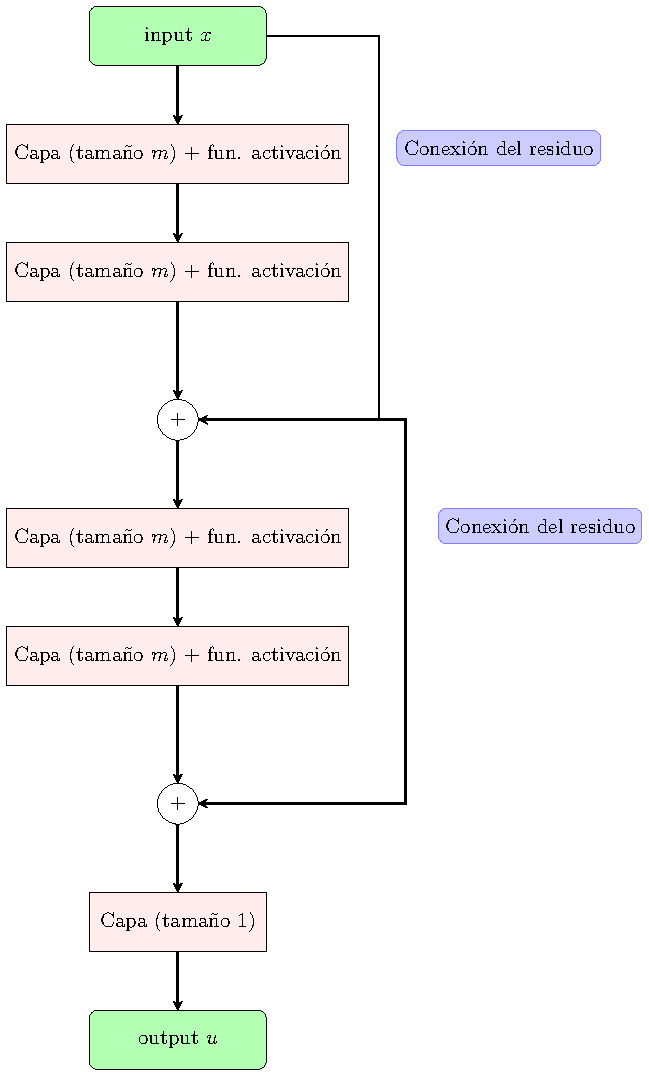
\includegraphics[width=0.5\textwidth]{TEX_Figures/deep_ritz_nn.pdf}
    \caption{La figura muestra una red con dos bloques y una capa lineal de salida.
    Cada bloque consiste en dos capas completamente conectadas y una conexión de salto.}
    \label{fig:net_structure_1}
\end{figure}
Dada una arquitectura de red \( \mathcal{N} \), el espacio de aproximación \( V_{\mathcal{N}} \) utilizado en el método Deep Ritz se define como:

\begin{equation*}
V_{\mathcal{N}} := \{ \hat{u}_\theta: \mathbb{R}^d \to \mathbb{R} \mid \theta \in \mathbb{R}^{\#\mathcal{N}} \}.
\end{equation*}

Mientras que \( \#\mathcal{N} \) sea finito y las funciones de activación sean diferenciables, se cumple que \( V_{\mathcal{N}} \subset H^1(\Omega) \). Sin embargo, en general, para \( u_{\mathcal{N}} \in V_{\mathcal{N}} \) no se garantiza que \( u_{\mathcal{N}} = 0 \) en \( \partial \Omega \), por lo que \( V_{\mathcal{N}} \not\subset V = H^1_0(\Omega) \). Además, es importante notar que \( V_{\mathcal{N}} \) no es un espacio vectorial, ya que para \( v_1, v_2 \in V_{\mathcal{N}} \) no necesariamente se cumple que \( v_1 + v_2 \in V_{\mathcal{N}} \).

Para abordar esta limitación, se introduce el funcional de energía penalizado:
\begin{equation*}
J_{\lambda}(v) := J(v) + \frac{\lambda}{2} |v|^2_{\partial \Omega},
\end{equation*}
donde \( \lambda \in \mathbb{R}^+ \) es un parámetro de penalización y \( | \cdot |_{\partial \Omega} \) denota la norma \( L^2 \) en la frontera del dominio. El término de penalización adicional impone que \( v \) sea próximo a cero en \( \partial \Omega \).

Esta formulación permite el uso de redes neuronales en la aproximación de ecuaciones diferenciales parciales sin necesidad de definir funciones de base explícitas, facilitando la resolución de problemas de altas dimensiones donde los métodos clásicos pueden volverse ineficientes. No obstante, igual que en el caso de las PINN el problema de la formulación residía en que se aproximaba el residuo de forma fuerte, en el método Deep Ritz, el problema radica en que se minimiza el funcional \( J_{\lambda} \) en lugar de \( J \), es decir, se altera el problema para imponer las condiciones de contorno, variando así la solución. Para ver esto de forma más clara, vamos a aplicar el método Deep Ritz a la ecuación de Poisson en una dimensión.


\begin{mdframed}  
    \begin{exmp}
        Consideremos la ecuación de Poisson en una dimensión, con $f = 1$ y $\Omega=(0,1)$
        \begin{equation}\label{eq:ejemplo_poisson}
        -u'' = 1, \quad u(0) = u(1) = 0,
        \end{equation} 
        cuya solución exacta es 
        \begin{equation*}
        u(x) = -x^2/2 + x/2.
        \end{equation*}
        En forma débil, la ecuación \eqref{eq:ejemplo_poisson} se puede escribir como: encontrar \( u \in H^1(0,1) \) tal que:
        \begin{equation*}
            \int_0^1 u'v' = \int_0^1 v \quad \forall v \in H^1(0,1).
        \end{equation*}
        en cuyo caso, la forma bilienal $a$ y lienal $l$ asociadas son:
        \begin{align*}
            a(u,v) &= \int_0^1 u'v', \\
            l(v) &= \int_0^1 v.
        \end{align*}
        Por lo tanto, el funcional \( J(u) \) asociado a este problema es:
        \begin{equation*}
            J(u) = \frac{1}{2} \int_0^1 (u')^2 - \int_0^1 u.
        \end{equation*}
        Con esta información podemos plantear el método de Ritz para este problema como encontrar \( \hat{u}_\theta \in V_{\mathcal{N}} \) tal que: 
        \begin{align*}
        \argmin_{\{\hat{u}_\theta:\; \theta \in \mathbb{R}^{\#\mathcal{N}} \}} \left( \frac{1}{2} \int_\Omega \left((\hat{u}_\theta')^2 - \int_\Omega \hat{u}_\theta + \lambda (\hat{u}_\theta(0)^2 + \hat{u}_\theta(1)^2)\right)\right) =\\
        \argmin_{\{\hat{u}_\theta:\; \theta \in \mathbb{R}^{\#\mathcal{N}} \}} \left(\frac{1}{2} \int_0^1 \left((\hat{u}_\theta')^2 - \int_0^1 \hat{u}_\theta + \lambda (\hat{u}_\theta(0)^2 + \hat{u}_\theta(1)^2)\right)\right),
        \end{align*}
        donde \(\hat{u}_\theta\) es una función de una red neuronal. Así, el funcional que estamos minimizando, $J_\lambda: H^1(0,1) \to \mathbb{R}$ se define como:
        \begin{equation*}
        J_\lambda(u) = \frac{1}{2} \int_0^1 \left((u')^2 - \int_0^1 u + \lambda (u(0)^2 + u(1)^2)\right).
        \end{equation*}
        Si buscamos el mínimo de \( J_\lambda \), vamos a encontrar que $u$ verifica la siguiente ecuación:
        \begin{equation*}
        J_\lambda'(u)v := \lim_{\beta \to 0} \frac{J_\lambda(u + \beta v) - J_\lambda(u)}{\beta} = 0, \qquad \forall v \in H^1(0,1).
        \end{equation*}
        Es fácil ver que \(u \in H^1(0,1)\) verifica
        \begin{equation*}
        \int_0^1 u'v' - \int_0^1 v + 2\lambda u(0)v(0) + 2\lambda u(1)v(1) = 0, \quad \forall v \in H^1(0,1).
        \end{equation*}
        Consideramos ahora el siguiente problema: encontrar \(u \in C^2(0,1)\) tal que 
        \begin{equation*}
        -u'' = f, \quad u'(0) = 2\lambda u(0), \quad u'(1) = -2\lambda u(1),
        \end{equation*}
        que tiene como solución para \(f = 1\)
        \begin{equation*}
        u_\lambda = -x^2/2 + x/2 + 1/(4\lambda).
        \end{equation*}
        La solución débil de este problema es: encontrar \(u \in H^1(0,1)\) tal que 
        \begin{equation*}
        \int_0^1 u'v' + 2\lambda u(1)v(1) + 2\lambda u(0)v(0) = \int_0^1 v, \quad \forall v \in H^1(0,1).
        \end{equation*}
        O lo que es lo mismo, encontrar \(u \in H^1(0,1)\) tal que 
        \begin{equation*}
        \int_0^1 u'v' + 2\lambda v(1)u(1) + 2\lambda v(0)u(0) = \int_0^1 v, \quad \forall v \in H^1(0,1).
        \end{equation*}
    \end{exmp}
\end{mdframed}
    
Con este ejemplo, nos damos cuenta de que el método Deep Ritz, en su formulación utilizada aquí, no aproxima exactamente el problema original, sino que en su lugar resuelve una ecuación con condiciones de frontera modificadas. Esto introduce un sesgo en la solución obtenida, lo que implica que el método no es exacto para el problema original de Poisson con condiciones de Dirichlet homogéneas. Siendo más específicos, el método Deep Ritz estaría aproximando la solución $u_\lambda(x) = -x^2/2 + x/2 + 1/(4\lambda)$ en lugar de la solución exacta $u(x) = -x^2/2 + x/2$, lo que implica un error de $O(1/\lambda)$ en la solución obtenida. 

A continuación, vamos a plantear la ecuación de Poisson en un dominio cuadrado y en una L, para lo cual he tenido que programar el método Deep Ritz en Python usando PyTorch. El objetivo con este ejemplo es entender cómo se comporta el método Deep Ritz ante los distintos valores que puede tomar el parámetro de penalización $\lambda$.

\begin{mdframed}
    \begin{exmp}
        Consideramos el siguiente problema de Poisson en un cuadrado unitario $\Omega = (0,1)^2$ con condiciones de contorno Dirichlet homogéneas:
        \begin{equation}\label{eq:poisson_square}
        \begin{cases}
        -\Delta u = 1, & \text{en } \Omega,\\
        u = 0, & \text{en } \partial \Omega.
        \end{cases}            
        \end{equation}
        Para aplicar el método, lo primero que necesitamos es definir el funcional $J_\lambda(u)$ asociado a este problema. Para ello lo primero que tenemos que hacer es obtener la forma débil de la ecuación. Sea \( v \) una función en el espacio de funciones \(H_0^1(\Omega) \), donde:
        \begin{equation*}
        H_0^1(\Omega) = \{ v \in H^1(\Omega) \mid v = 0 \text{ en } \partial \Omega \}.
        \end{equation*}
        Multiplicamos la ecuación diferencial por $v$ e integramos en \(\Omega\):
        \begin{equation*}
        \int_{\Omega} (-\Delta u) v \,dx = \int_{\Omega} 1 \cdot v \,dx.
        \end{equation*}
        Integramos por partes:
        \begin{equation*}
        \int_{\Omega} (-\Delta u) v \,dx = \int_{\Omega} \nabla u \cdot \nabla v \,dx - \int_{\partial\Omega} \frac{\partial u}{\partial n} v \,ds.
        \end{equation*}
        Dado que \( v = 0 \) en \( \partial \Omega \), el término de la frontera desaparece, dejando la forma débil:
        \begin{equation*}
        \int_{\Omega} \nabla u \cdot \nabla v \,dx = \int_{\Omega} v \,dx, \quad \forall v \in H_0^1(\Omega).
        \end{equation*}
        El funcional asociado a este problema se define como:
        \begin{equation*}
        J(u) = \frac{1}{2} \int_{\Omega} |\nabla u|^2 \,dx - \int_{\Omega} u \,dx.
        \end{equation*}
        Así, el funcional $J_\lambda(u)$ se define como:
        \begin{equation*}
        J_\lambda(u) = \frac{1}{2} \int_\Omega |\nabla u|^2 - \int_\Omega u + \lambda \int_{\partial \Omega} u^2.
        \end{equation*}
        Para resolver este problema, implementé el método Deep Ritz en Python con PyTorch. La red neuronal que usé tiene la arquitectura 2-64-64-1. En la Figura \ref{fig:poisson_square} se muestra la solución obtenida con $\lambda=500$, y en la Figura \ref{fig:diferencia_cuadrado} se compara con la solución del método de elementos finitos. Se observa que la solución obtenida con el método Deep Ritz presenta diferencias significativas con respecto a la del método de los elementos finitos. De hecho, este resultado, a pesar de ser de los mejores que se pueden lograr con Deep Ritz en este problema, sigue estando lejos de la solución real.

        Siguiendo la intuición del caso unidimensional, al reducir $\lambda$ a $10^5$, esperamos una aproximación mucho peor. Y, efectivamente, la solución resultante no se parece en nada a la real. La Figura \ref{fig:poisson_square_lambda_1e-5} muestra este resultado.

        \begin{figure}[H]
            \centering
            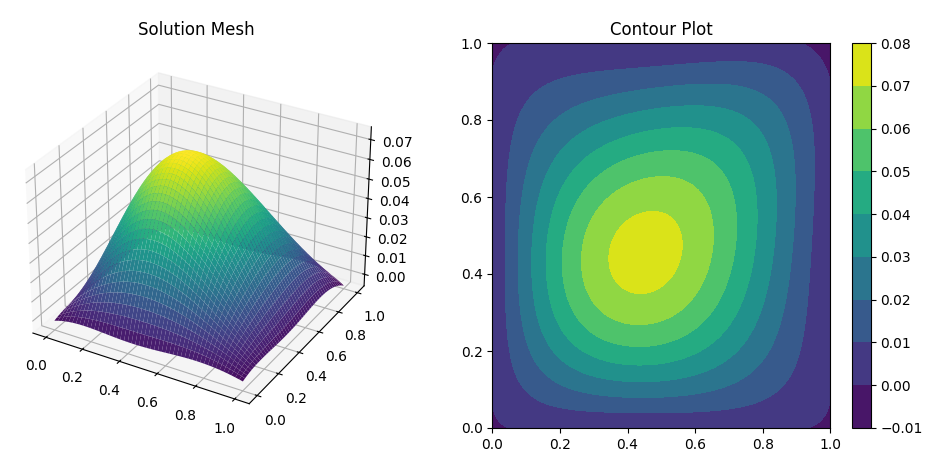
\includegraphics[width=1\textwidth]{Figuras/PoissonSquareBien.png}
            \caption{Solución de la ecuación de Poisson en un cuadrado unitario con $\lambda = 500$.}
            \label{fig:poisson_square}
        \end{figure}

        \begin{figure}[H]
            \centering
            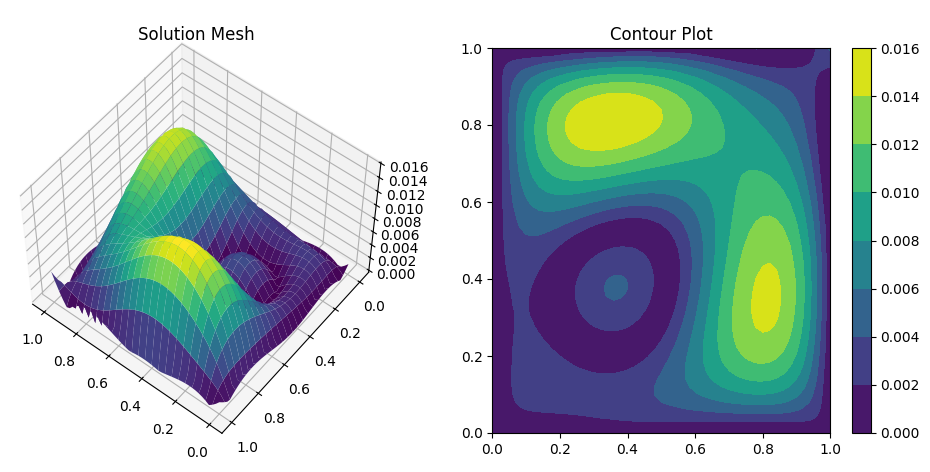
\includegraphics[width=1\textwidth]{Figuras/DiferenciaCuadrado.png}
            \caption{Diferencia entre FEM y Deep Ritz con $\lambda = 500$.}
            \label{fig:diferencia_cuadrado}
        \end{figure}

        \begin{figure}[H]
            \centering
            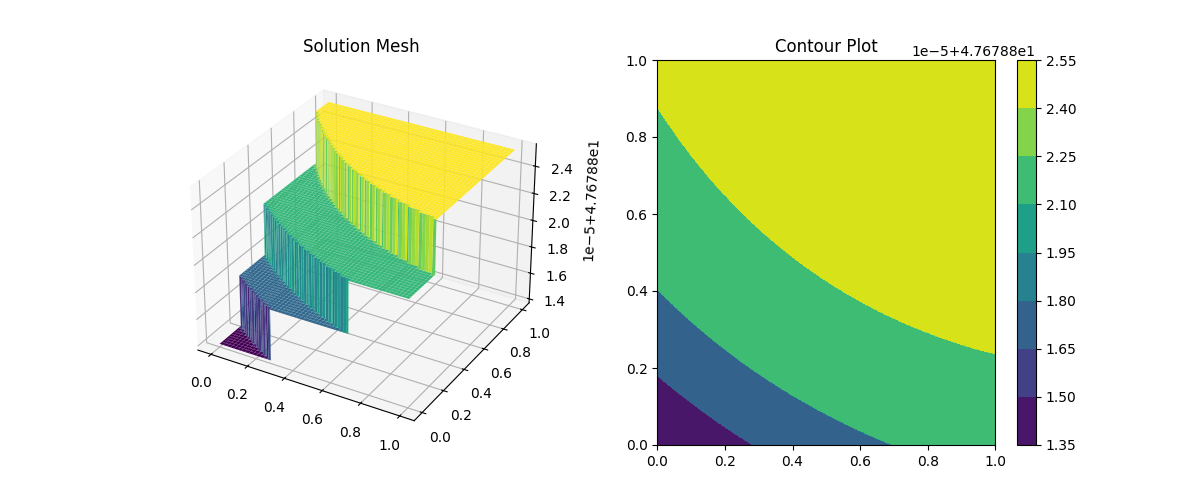
\includegraphics[width=1\textwidth]{Figuras/PoissonSquare10e-5.png}
            \caption{Solución de la ecuación de Poisson en un cuadrado unitario con $\lambda = 10^{-5}$.}
            \label{fig:poisson_square_lambda_1e-5}
        \end{figure}

        El código que se ha utilizado para implementar el método Deep Ritz en este problema se puede encontrar en el Anexo \ref{sec:codigo_deep_ritz}.
    \end{exmp}
\end{mdframed}

El método Deep Ritz ofrece una formulación efectiva para superar las limitaciones de las PINN tradicionales, que imponen el residuo en forma fuerte. Sin embargo, como se ha ilustrado en los ejemplos, la manera en que este método maneja las condiciones de contorno no es del todo óptima. En particular, el uso de un término de penalización para forzar el cumplimiento de las condiciones de frontera introduce una modificación en el problema original, lo que puede generar soluciones sesgadas, especialmente cuando el parámetro de penalización $\lambda$ no es suficientemente grande.

En comparación con el método de elementos finitos (FEM), el Deep Ritz tiene la ventaja de no requerir la construcción explícita de funciones base, lo que resulta especialmente útil en problemas de alta dimensionalidad. No obstante, esta misma característica es también una limitación, ya que, en el FEM, las funciones base garantizan automáticamente el cumplimiento de las condiciones de contorno, mientras que en el método Deep Ritz esto debe ser impuesto externamente, con los problemas asociados que hemos analizado.

\chapter{Conclusiones}\label{chap4}

El uso de redes neuronales para la aproximación de ecuaciones en derivadas parciales es un campo con un gran potencial teórico. Su capacidad de aproximar funciones complejas y de operar en dimensiones altas sin la necesidad de una malla explícita las hace atractivas en escenarios donde los métodos numéricos tradicionales pueden resultar costosos o impracticables. No obstante, en la práctica, su aplicación a problemas relativamente simples muestra importantes deficiencias en comparación con métodos bien establecidos como el método de los elementos finitos (FEM).

Los enfoques basados en redes neuronales, como las PINNs (Physics-Informed Neural Networks), presentan limitaciones importantes al forzar el cumplimiento de la ecuación diferencial en su forma fuerte. Esto implica que, en situaciones donde no existe una solución en este sentido, la red neuronal no puede aproximar correctamente la solución débil. Además, la falta de garantías de convergencia y la ausencia de una base matemática sólida para la selección de hiperparámetros complican su aplicación efectiva.

Por otro lado, el método Deep Ritz plantea una alternativa más alineada con la formulación variacional de los problemas elípticos, minimizando un funcional en lugar de imponer restricciones puntuales. Sin embargo, el uso de penalizaciones para imponer condiciones de contorno introduce modificaciones en el problema original, lo que afecta la precisión de la solución obtenida. A pesar de ello, este enfoque podría ser más viable en problemas de alta dimensionalidad, donde los métodos tradicionales pierden eficiencia.

En resumen, aunque las redes neuronales ofrecen herramientas novedosas para la resolución de ecuaciones diferenciales, su aplicación en contextos prácticos aún enfrenta numerosos desafíos. Su rendimiento es inferior al de métodos numéricos establecidos en escenarios convencionales, y la interpretabilidad de los resultados sigue siendo limitada. La dificultad para diagnosticar fallos y la falta de garantías teóricas claras refuerzan la idea de que, por el momento, estas técnicas deben verse como complementarias a los métodos clásicos, en lugar de como un reemplazo directo.

\appendix   
\chapter{Código en Matlab para la red neuronal de clasificación\label{sec:codigo_clasificacion}}

El código aquí escrito está basado en el propuesto por Catherine et al. en \cite{deeplearningSIAM} pero extendiéndolo para incluir más puntos de entrenamiento de distinto tipo.

Lo primero que se hace es declarar cada punto de entrenamiento y su respectiva etiqueta. En este caso, las etiquetas son vectores de 3 componentes, donde cada componente representa la probabilidad de que el punto pertenezca a una de las tres clases. 

\begin{lstlisting}[language=Matlab]
function pclassifier_more_points

% xcoords, ycoords, targets
x1 = [0.1,0.3,0.1,0.2,0.4,0.6,0.5,0.9,0.4,0.7,0.3,0.4,0.2,0.1,0.5, 0.9,0.8];
x2 = [0.1,0.4,0.5,0.2,0.2,0.3,0.6,0.2,0.4,0.6,0.9,0.7,0.6,0.8,0.8, 0.6,0.1];
y = [ones(1,5) zeros(1,11) 1; zeros(1,5) ones(1,5) zeros(1,7); zeros(1,10) ones(1,6) 0];
\end{lstlisting}

A continuación, visualizamos los puntos creados. En este caso, la primera clase esta representada por círculos rojos, la segunda por cruces azules y la tercera por triángulos verdes.

\begin{lstlisting}[language=Matlab]
figure(1)
clf
a1 = subplot(1,1,1);
plot(x1(1:5),x2(1:5),'ro','MarkerSize',12,'LineWidth',4)
hold on
plot(x1(17),x2(17),'ro','MarkerSize',12,'LineWidth',4)
plot(x1(6:10),x2(6:10),'bx','MarkerSize',12,'LineWidth',4)
plot(x1(11:16),x2(11:16),'gv','MarkerSize',12,'LineWidth',4)
a1.XTick = [0 1];
a1.YTick = [0 1];
a1.FontWeight = 'Bold';
a1.FontSize = 10;
xlim([0,1])
ylim([0,1])

print -dpng pic_more_points.png

\end{lstlisting}

Es siguiente paso es crear las matrices de pesos y sesgos que van a definir la red neuronal. En este caso, la red tiene 2 capas ocultas y una capa de salida. La primera capa oculta tiene 2 neuronas, la segunda 3 y la capa de salida 3 neuronas.

\begin{lstlisting}[language=Matlab]

rng(5000);
W2 = 0.5*randn(2,2);
W3 = 0.5*randn(3,2);
W4 = 0.5*randn(3,3);
b2 = 0.5*randn(2,1);
b3 = 0.5*randn(3,1);
b4 = 0.5*randn(3,1);

\end{lstlisting}

Finalmente, queda el paso de entrenamiento de la red neuronal. Este sigue el algoritmo de retropropagación, donde se calcula el gradiente del coste y se actualizan los pesos y sesgos de la red. 

\begin{lstlisting}[language=Matlab]
eta = 0.05;
Niter = 1e6;
savecost = zeros(Niter,1);
for counter = 1:Niter
    k = randi(17);
    x = [x1(k); x2(k)];
    % Forward pass
    a2 = activate(x,W2,b2);
    a3 = activate(a2,W3,b3);
    a4 = activate(a3,W4,b4);
    % Backward pass
    delta4 = a4.*(1-a4).*(a4-y(:,k));
    delta3 = a3.*(1-a3).*(W4'*delta4);
    delta2 = a2.*(1-a2).*(W3'*delta3);
    % Gradient step
    W2 = W2 - eta*delta2*x';
    W3 = W3 - eta*delta3*a2';
    W4 = W4 - eta*delta4*a3';
    b2 = b2 - eta*delta2;
    b3 = b3 - eta*delta3;
    b4 = b4 - eta*delta4;
    % Monitor progress
    newcost = cost(W2,W3,W4,b2,b3,b4);   % display cost to screen
    savecost(counter) = newcost;
end

\end{lstlisting}

Acabado el entrenamiento, el paso final es visualizar los resultados, para ver que regiones asigna la red neuronal a cada una de las clases existentes.

\begin{lstlisting}[language=Matlab]
figure(2)
clf
semilogy(1:1e4:Niter,savecost(1:1e4:Niter),'b-','LineWidth',2)
xlabel('Iteration Number')
ylabel('Value of cost function')
set(gca,'FontWeight','Bold','FontSize',10)
print -dpng pic_cost_more_points.png

%%%%%%%%%%% Display shaded and unshaded regions 
N = 500;
Dx = 1/N;
Dy = 1/N;
xvals = 0:Dx:1;
yvals = 0:Dy:1;
for k1 = 1:N+1
    xk = xvals(k1);
    for k2 = 1:N+1
        yk = yvals(k2);
        xy = [xk;yk];
        a2 = activate(xy,W2,b2);
        a3 = activate(a2,W3,b3);
        a4 = activate(a3,W4,b4);
        Aval(k2,k1) = a4(1);
        Bval(k2,k1) = a4(2);
        Cval(k2,k1) = a4(3);
     end
end
[X,Y] = meshgrid(xvals,yvals);

figure(3)
clf
a2 = subplot(1,1,1);

Mval = ones(size(Aval));

Mval(Cval >= Aval & Cval >= Bval) = 2;
Mval(Aval >= Bval & Aval >= Cval) = 1;
Mval(Bval >= Aval & Bval >= Cval) = 0;

contourf(X, Y, Mval, [-1 0.75 1.5 2.5]); 

hold on

colormap([1 1 1; 0.8 0.8 0.8; 0.5 0.5 0.5]);

plot(x1(1:5),x2(1:5),'ro','MarkerSize',12,'LineWidth',4)
plot(x1(17),x2(17),'ro','MarkerSize',12,'LineWidth',4)
plot(x1(6:10),x2(6:10),'bx','MarkerSize',12,'LineWidth',4)
plot(x1(11:16),x2(11:16),'yv','MarkerSize',12,'LineWidth',4)
a2.XTick = [0 1];
a2.YTick = [0 1];
a2.FontWeight = 'Bold';
a2.FontSize = 10;
xlim([0,1])
ylim([0,1])

print -dpng classifier_back_more_points.png

  function costval = cost(W2,W3,W4,b2,b3,b4)

     costvec = zeros(10,1); 
     for i = 1:10
         x =[x1(i);x2(i)];
         a2 = activate(x,W2,b2);
         a3 = activate(a2,W3,b3);
         a4 = activate(a3,W4,b4);
         costvec(i) = norm(y(:,i) - a4,2);
     end
     costval = norm(costvec,2)^2;
   end % of nested function

end
\end{lstlisting}


\chapter{Código en Python para el método de los elementos finitos en un cuadrado\label{sec:codigo_fem_cuadrado}}

El primer paso consiste en definir la malla sobre la que se realizará la aproximación. Se elige un número de puntos en cada dirección, denotado como $n$, y se calcula el tamaño del paso $h = 1/n$. Esto permite dividir el dominio $\Omega = [0,1] \times [0,1]$ en una malla uniforme.

\begin{lstlisting}[language=Python] 
import numpy as np
import scipy.sparse as sp
import scipy.sparse.linalg as spla
import matplotlib.pyplot as plt

n = 50
h = 1 / n
\end{lstlisting}

El siguiente paso es definir la matriz de coeficientes del sistema lineal, que representa la discretización del operador diferencial en la malla. Se utiliza una combinación de matrices tridiagonales y productos de Kronecker para construir la estructura del problema.

\begin{lstlisting}[language=Python] 
e = np.ones(n-1)
B = sp.diags([-e, 4*e, -e], [-1, 0, 1], shape=(n-1, n-1))
I = sp.eye(n-1)
I1 = sp.diags([-e, -e], [-1, 1], shape=(n-1, n-1))
A = sp.kron(I, B) + sp.kron(I1, I)
A /= h**2
\end{lstlisting}

Se define el término independiente del sistema, que en este caso es un vector lleno de unos en todo el dominio, excepto en la frontera. Esto refleja que la solución aproximada debe tomar el valor $1$ en cada punto interior de la malla y $0$ en la frontera.

\begin{lstlisting}[language=Python] 
f = np.ones((n-1)**2)
\end{lstlisting}

Para obtener la solución, se resuelve el sistema lineal $A y = f$ utilizando la función \texttt{spsolve} de la librería \texttt{scipy}. El resultado se almacena en la variable $y$.

\begin{lstlisting}[language=Python] 
y = spla.spsolve(A, f)
\end{lstlisting}

Finalmente, la solución se reorganiza en una matriz para representarla gráficamente. Se muestran dos visualizaciones: una malla tridimensional y un gráfico de contorno, que permiten interpretar mejor la distribución de valores obtenidos.

\begin{lstlisting}[language=Python] 
val = np.zeros((n-1, n-1))
for i in range(n-1):
    for j in range(n-1):
        val[i, j] = y[j + (n-1) * i]

valnn = np.zeros((n+1, n+1))
valnn[1:n, 1:n] = val

xx = np.linspace(0, 1, n+1)
yy = xx
X, Y = np.meshgrid(xx, yy)

fig = plt.figure(figsize=(12, 5))

ax1 = fig.add_subplot(121, projection='3d')
ax1.plot_surface(X, Y, valnn, cmap='viridis')
ax1.set_title('Solution Mesh')

ax2 = fig.add_subplot(122)
c = ax2.contourf(X, Y, valnn, cmap='viridis')
plt.colorbar(c, ax=ax2)
ax2.set_title('Contour Plot')

plt.show()
\end{lstlisting}


\chapter{Código en Python para construir PINNs con la librería DeepXDE\label{sec:codigo_pinns}}

El siguiente código es el utilizado en el ejemplo \ref{exmp:fallo}. Lo primero que se hace es importar las librerias necesarias para el funcionamiento del código. En este caso, se utilizan las librerías de DeepXDE para la implementación de la red neuronal y Matplotlib para la visualización. Además, se define el ecuación en derivadas parciales (EDP) que se va a resolver. 

\begin{lstlisting}[language=Python]
import deepxde as dde
import matplotlib.pyplot as plt
import numpy as np
import tensorflow as tf 

def pde(x, u):
    A = 0.5 * tf.cast(tf.less(x, 0), tf.float32) + 1 * tf.cast(tf.greater_equal(x, 0), tf.float32) 
    du_x = dde.grad.jacobian(u, x) 
    dA_du_x = dde.grad.jacobian(A * du_x, x) 
    f = 0 * tf.cast(tf.less(x, 0), tf.float32) + (-2) * tf.cast(tf.greater_equal(x, 0), tf.float32) 
    return -dA_du_x - f

\end{lstlisting}

A continueación se define el solución débil de la EDP, que se utilizará como referencia para evaluar el rendimiento de la red neuronal. Además, se definen las condiciones de frontera. En este caso, se utiliza una condición de Dirichlet en la frontera del dominio.

\begin{lstlisting}[language=Python]
def weak_solution(x):
    return (-2/3 * x - 2/3) * (x < 0) + (x**2 - (1/3) * x - (2/3)) * (x >= 0)

def boundary(x, on_boundary):
    return on_boundary
    
geom = dde.geometry.Interval(-1, 1)
bc = dde.DirichletBC(geom, weak_solution, boundary)
\end{lstlisting}

Seguidamente, definimos el objeto red neuronal que se va a utilizar para aproximar la solución de la EDP así como el método de optimización. 

\begin{lstlisting}[language=Python]
data = dde.data.PDE(geom, pde, bc, num_domain=1000, num_boundary=2, num_test=100, solution=weak_solution)

net = dde.maps.FNN([1] + [256] * 3 + [1], "tanh", "Glorot normal")

model = dde.Model(data, net)

model.compile("adam", lr=0.001,metrics=["l2 relative error"])
\end{lstlisting}

Con todos los parámetros del problema definidos, nos apoyamos en el método \texttt{train} de la librería DeepXDE para entrenar la red neuronal. 

\begin{lstlisting}[language=Python]
losshistory, train_state = model.train(iterations=10000)
\end{lstlisting}

Finalmnte, se guarda el historial de pérdidas y se visualiza la solución aproximada. Se generan 1000 puntos uniformemente distribuidos en el intervalo \([-1, 1]\) y se evalúa la red neuronal en esos puntos. Luego, se grafican los resultados.

\begin{lstlisting}[language=Python]
dde.saveplot(losshistory, train_state, issave=True, isplot=True)

x = geom.uniform_points(1000, True)
y = model.predict(x, operator=pde)
plt.figure()
plt.plot(x, y)
plt.xlabel("x")
plt.ylabel("Residuo de la EDP")
plt.show()
\end{lstlisting}


\chapter{Código en Python método DeepRitz\label{sec:codigo_deep_ritz}}

Este código implementa una red neuronal para resolver ecuaciones en derivadas parciales mediante el método de Ritz. Se describe la construcción del modelo, el proceso de entrenamiento y la evaluación de la solución.

Se importan las bibliotecas necesarias para realizar gráficas, implementar redes neuronales en PyTorch y realizar operaciones matemáticas.

\begin{lstlisting}[language=Python]
import numpy as np 
import math, torch, generateData, time
import torch.nn.functional as F
from torch.optim.lr_scheduler import MultiStepLR, StepLR
import torch.nn as nn
import matplotlib.pyplot as plt
import sys, os
import writeSolution
import numpy as np
import scipy.sparse as sp
import scipy.sparse.linalg as spla
import matplotlib.pyplot as plt
\end{lstlisting}

Se define la clase \texttt{RitzNet}, que implementa una red neuronal profunda para aproximar soluciones.

\begin{lstlisting}[language=Python]
class RitzNet(torch.nn.Module):
    def __init__(self, params):
        super(RitzNet, self).__init__()
        self.params = params
        self.linearIn = nn.Linear(self.params["d"], self.params["width"])
        self.linear = nn.ModuleList()
        for _ in range(params["depth"]):
            self.linear.append(nn.Linear(self.params["width"], self.params["width"]))

        self.linearOut = nn.Linear(self.params["width"], self.params["dd"])

    def forward(self, x):
        x = torch.tanh(self.linearIn(x)) 
        for layer in self.linear:
            x_temp = torch.tanh(layer(x))
            x = x_temp
        
        return self.linearOut(x)

\end{lstlisting}

Se define el proceso de entrenamiento de la red neuronal mediante el método de optimización de Adam.

\begin{lstlisting}[language=Python]
def train(model,device,params,optimizer,scheduler):
    ratio = (4*2.0+2*math.pi*0.3)/(2.0*2.0-math.pi*0.3**2)
    model.train()

    data1 = torch.from_numpy(generateData.sampleFromSquare(1,params["bodyBatch"])).float().to(device)
    data2 = torch.from_numpy(generateData.sampleFromSquareBoundary(1,params["bdryBatch"])).float().to(device)
    x_shift = torch.from_numpy(np.array([params["diff"],0.0])).float().to(device)
    y_shift = torch.from_numpy(np.array([0.0,params["diff"]])).float().to(device)
    data1_x_shift = data1+x_shift
    data1_y_shift = data1+y_shift

    loss_history = []  

    for step in range(params["trainStep"]-params["preStep"]):
        output1 = model(data1)
        output1_x_shift = model(data1_x_shift)
        output1_y_shift = model(data1_y_shift)

        dfdx = (output1_x_shift-output1)/params["diff"]
        dfdy = (output1_y_shift-output1)/params["diff"]

        model.zero_grad()

        
        fTerm = ffun(data1).to(device)
        loss1 = torch.mean(0.5*(dfdx*dfdx+dfdy*dfdy)-fTerm*output1)

        
        output2 = model(data2)
        target2 = exact(data2)
        loss2 = torch.mean((output2-target2)*(output2-target2) * params["penalty"] * ratio)
        loss = loss1+loss2              
        loss_history.append(loss.item())  

        if step%params["writeStep"] == params["writeStep"]-1:
            with torch.no_grad():
                target = exact(data1)
                error = errorFun(output1,target,params)
                
                print("Loss at Step %s is %s."%(step+params["preStep"]+1,loss.item()))
            file = open("lossData.txt","a")
            file.write(str(step+params["preStep"]+1)+" "+str(error)+"\n")

        if step%params["sampleStep"] == params["sampleStep"]-1:
            data1 = torch.from_numpy(generateData.sampleFromSquare(1, params["bodyBatch"])).float().to(device)
            data2 = torch.from_numpy(generateData.sampleFromSquareBoundary(1, params["bdryBatch"])).float().to(device)

            data1_x_shift = data1+x_shift
            data1_y_shift = data1+y_shift

        if 10*(step+1)%params["trainStep"] == 0:
            print("%s%% finished..."%(100*(step+1)//params["trainStep"]))

        loss.backward()

        optimizer.step()
        scheduler.step()

    return loss_history  

\end{lstlisting}

Se incluyen funciones para calcular el error y visualizar la evolución de la pérdida durante el entrenamiento.

\begin{lstlisting}[language=Python]
def errorFun(output, target, params):
    error = output - target
    error = math.sqrt(torch.mean(error * error))
    ref = math.sqrt(torch.mean(target * target))
    
    if ref == 0:  
        return error  
    
    return error / ref  

def test(model, device, params):
    numQuad = params["numQuad"]

    data = torch.from_numpy(generateData.sampleFromSquare(1,numQuad)).float().to(device)
    output = model(data)
    target = exact(data).to(device)

    error = output - target
    error = math.sqrt(torch.mean(error * error))
    ref = math.sqrt(torch.mean(target * target))

    if ref == 0:  
        return error  

    return error / ref

def ffun(data):
    return torch.ones([data.shape[0],1],dtype=torch.float)

def exact(data):
    return torch.zeros((data.shape[0], 1), dtype=torch.float, device=data.device)


def count_parameters(model):
    return sum(p.numel() for p in model.parameters())

def plot_loss(loss_history):
    plt.figure(figsize=(8, 6))
    plt.plot(range(len(loss_history)), loss_history, linestyle='-')
    plt.xlabel("Iterations (every {} steps)".format(500))
    plt.ylabel("Loss")
    plt.yscale("log")  
    plt.title("Training Loss Over Time (Log Scale)")
    plt.grid(True, which="both", linestyle="--", linewidth=0.5)  
    plt.show()
\end{lstlisting}

La función \texttt{principal} define los parámetros, inicializa la red, ejecuta el entrenamiento y evaluación y grafica los resultados. Los parámetros utilizados tienen el siguiente significado:
\begin{itemize}
    \item \texttt{d}: Dimensionalidad del problema (2 para el cuadrado).
    \item \texttt{dd}: Dimensionalidad de la salida (1 para un escalar).
    \item \texttt{bodyBatch}: Tamaño del lote para el cuerpo.
    \item \texttt{bdryBatch}: Tamaño del lote para la frontera.
    \item \texttt{lr}: Tasa de aprendizaje.
    \item \texttt{width}: Ancho de la red neuronal.
    \item \texttt{depth}: Profundidad de la red neuronal.
    \item \texttt{numQuad}: Número de puntos de colocación.
    \item \texttt{trainStep}: Número total de pasos de entrenamiento.
    \item \texttt{penalty}: Parámetro de penalización.
    \item \texttt{preStep}: Pasos previos al entrenamiento principal.
    \item \texttt{diff}: Diferencia utilizada en el cálculo del gradiente.
\end{itemize}

\begin{lstlisting}
def main():
    
    device = torch.device("cuda:0" if torch.cuda.is_available() else "cpu")

    params = dict()
    params["d"] = 2 
    params["dd"] = 1 
    params["bodyBatch"] = 1024 
    params["bdryBatch"] = 1024 
    params["lr"] = 0.0001 
    params["width"] = 64 
    params["depth"] = 4 
    params["numQuad"] = 40000 
    params["trainStep"] = int(1e4)
    params["penalty"] = 500
    params["preStep"] = 0
    params["diff"] = 0.001
    params["writeStep"] = 500
    params["sampleStep"] = 10
    params["step_size"] = 5000
    params["gamma"] = 0.3
    params["decay"] = 0.00001

    startTime = time.time()
    model = RitzNet(params).to(device)
    print("Generating network costs %s seconds."%(time.time()-startTime))

    preOptimizer = torch.optim.Adam(model.parameters(),lr=params["preLr"])
    optimizer = torch.optim.Adam(model.parameters(),lr=params["lr"],weight_decay=params["decay"])
    scheduler = StepLR(optimizer,step_size=params["step_size"],gamma=params["gamma"])

    startTime = time.time()
    loss_history = train(model,device,params,optimizer,scheduler)
    print("Training costs %s seconds."%(time.time()-startTime))

    model.eval()
    testError = test(model,device,params)
    print("The test error (of the last model) is %s."%testError)
    print("The number of parameters is %s,"%count_parameters(model))

    torch.save(model.state_dict(), "last_model.pt")

    
    plot_loss(loss_history)

    pltResult(model, device, 500)

    valn = femPoissonSquare(50)

    compare_fem_model(50, model, valn)
\end{lstlisting}


\printbibliography
\cleardoublepage


\end{document}
